\documentclass[10pt]{article}

\ifdefined\USEPREPRINT
  \usepackage[preprint]{tmlr}
\else
  \usepackage{tmlr}
\fi

% Note: tmlr.sty loads fontenc, lmodern, fancyhdr, and natbib (authoryear).
% Do not load geometry, lmodern, or pass numbers to natbib.
\usepackage{iftex}
\ifPDFTeX
  \usepackage[utf8]{inputenc}
\fi
\usepackage{microtype}
\usepackage{amsmath,amssymb,amsthm,mathtools,bm}
\usepackage{booktabs}
\usepackage{graphicx}
\usepackage{xcolor}
\usepackage{enumitem}
\usepackage[ruled,vlined,linesnumbered]{algorithm2e}
\usepackage{hyperref}
\usepackage[capitalize,noabbrev]{cleveref}

\hypersetup{
    colorlinks=true,
    linkcolor=blue!60!black,
    citecolor=green!50!black,
    urlcolor=blue!70!black
}

\graphicspath{{figures/}{../figures/}}

\crefname{algocf}{Algorithm}{Algorithms}
\Crefname{algocf}{Algorithm}{Algorithms}

\theoremstyle{plain}
\newtheorem{theorem}{Theorem}
\newtheorem{proposition}{Proposition}
\newtheorem{lemma}{Lemma}
\newtheorem{corollary}{Corollary}

\theoremstyle{definition}
\newtheorem{definition}{Definition}
\newtheorem{assumption}{Assumption}

\theoremstyle{remark}
\newtheorem{remark}{Remark}

\newcommand{\R}{\mathbb{R}}
\newcommand{\E}{\mathbb{E}}
\newcommand{\Prob}{\mathbb{P}}
\newcommand{\Var}{\operatorname{Var}}
\newcommand{\Cov}{\operatorname{Cov}}
\newcommand{\KL}{\operatorname{kl}}
\newcommand{\DKL}{D_{\mathrm{KL}}}
\newcommand{\TV}{\operatorname{TV}}
\newcommand{\SNR}{\operatorname{SNR}}
\newcommand{\logit}{\operatorname{logit}}
\newcommand{\ind}{\mathbf{1}}
\newcommand{\Fmix}{F_{\mathrm{mix}}}
\newcommand{\barFmix}{\bar{F}_{\mathrm{mix}}}
\newcommand{\fmix}{f_{\mathrm{mix}}}

\title{Joint Calibration--Compute Limits of Best-of-$N$ Scaling:\\
Minimax Theory, Prompt Heterogeneity, and an Empirical Audit}

\ifdefined\USEPREPRINT
\author{\name Xinkang Zhang \email 3203235490@qq.com \\
      \addr Independent Researcher}
\else
\author{\name Anonymous Authors}
\fi

\def\month{MM}
\def\year{YYYY}
\def\openreview{\url{https://openreview.net/forum?id=XXXX}}

\begin{document}

\maketitle

\begin{abstract}
Best-of-$N$ ($\mathrm{BoN}$) inference scaling degrades when heavy wrong-answer tails invert high verifier scores. Post-hoc calibration restores monotonicity for a fixed distribution, yet deployment faces finite offline labels ($M$), finite online candidates ($N$), and heterogeneous prompt mixtures $X \sim \mathcal{P}_X$. This paper establishes tight theoretical limits and audits when calibration helps or hurts. First, on uniformly $\beta$-smooth peaks, we prove that joint minimax excess accuracy regret decouples as $\Theta\big((\frac{\ln M}{M})^{\frac{\beta}{2\beta+1}} + N^{-\beta}\big)$, attained by $N$-agnostic equal-frequency $\mathrm{KL\text{-}LCB}$ with balance threshold $N_{\mathrm{balance}}(M) \asymp (M/\ln M)^{\frac{1}{2\beta+1}}$, and extend the rate to unknown marginals for all $\beta > 0$ via sample-split spacings. Second, under prompt heterogeneity, we decompose excess regret into cross-prompt pooling misspecification plus finite-$(M,N)$ estimation error, derive exact Simpson slope masking, prove a tight $N=2$ rank ceiling, and analyze prompt-wise online sample Z-scores $Z_{i,N}$ for homoscedastic Gaussian verifiers with general boundary prompt masses $(\pi_0, \pi_1) \in [0,1]^2$ and positive interior solvable mass on $[p_{\min}, p_{\max}] \subset (0, 1)$: $Z_{i,N}$ converges at $O_p(\sqrt{(\ln N)/N})$, tends at both tails to $\frac{\pi_1}{\pi_0+\pi_1}$, achieves zero ceiling loss when $\pi_0 = 0, \pi_1 > 0$ under right-half ($Z \ge 0$) monotonicity (avoiding an unconstrained left-tail overtake artifact), and incurs an affine-invariant ceiling loss below $\mathrm{Raw\text{-}BoN}$ whenever unsolvable prompts ($\pi_0 > 0$) and interior prompts coexist. Across five benchmark--verifier evaluation settings and an auxiliary multi-verifier correlation benchmark ($>1.03\times 10^6$ trajectories), an empirical audit shows that a minimal holdout gate ($\mathrm{Hybrid\text{-}Fixed}$) defaults to $\mathrm{Raw\text{-}BoN}$ on every clean benchmark ($0.00\,\mathrm{pp}$ clean-data gain), serving strictly as a risk-control baseline against Simpson confounding ($+2.41\,\mathrm{pp}$ on \texttt{S3}; $+1.83\,\mathrm{pp}$ on \texttt{RB2}) and Z-score ceiling drops ($-0.92$ to $-8.69\,\mathrm{pp}$), while counterfactual $\hat{\pi}_0 = 0$ filtering and distribution-shift matrices expose how low-prior hard prompts sustain tail inversion and where support clipping fails under in-support shifts.
\end{abstract}

\section{Introduction}
\label{sec:intro}

Sampling $N$ candidate solutions and selecting the top candidate according to an outcome reward model (RM) or process reward model (PRM) improves LLM reasoning without additional training \citep{cobbe2021training,wang2023selfconsistency,lightman2024lets,brown2024large,snell2024scaling,wu2024inference}. However, standard Best-of-$N$ ($\mathrm{BoN}$) probes the extreme upper tail $S_{(N)} = \max_{1\le i\le N} S_i$, where approximate verifiers and heavy wrong-answer tails trigger \emph{verifier overoptimization}: expected accuracy peaks at a finite compute budget and degrades as $N$ grows further \citep{gao2023scaling,stroebl2024inference,beirami2025theoretical,huang2025best,dorner2025roc,yano2026tail,gui2026whether}. For a single fixed distribution, ranking by the population posterior $q(s) = \Prob(Y=1 \mid S=s)$ restores monotonic scaling. Practical deployment, however, raises four sharper questions that determine whether post-hoc calibration actually improves upon uncalibrated $\mathrm{BoN}$:
\begin{enumerate}[leftmargin=1.5em,itemsep=1pt,topsep=1pt]
    \item Under $M$ offline labeled candidates and $N$ online unlabeled candidates, what is the minimax optimal excess regret $\mathcal{R}^*(M, N)$, and when does scaling compute $N$ saturate offline calibration capacity $M$?
    \item When offline calibration pools candidates across heterogeneous prompts $X \sim \mathcal{P}_X$, how do cross-prompt misspecification and finite-$(M,N)$ estimation errors decouple, and when does pooled calibration fail catastrophically via Simpson confounding?
    \item Does prompt-wise online sample Z-standardization $Z_{i,N}$ solve cross-prompt scaling distortion, or does boundary-prompt competition ($\pi_0$ unsolvable and $\pi_1$ trivial prompts) create an irreducible ceiling loss?
    \item On real modern LLM/RM benchmarks with little natural overoptimization, should practitioners deploy post-hoc calibration or leave $\mathrm{BoN}$ uncalibrated, and what happens under unseen out-of-support vs.\ in-support distribution shifts?
\end{enumerate}

\paragraph{Contributions and Framing.}
Rather than proposing another heuristic verifier wrapper, we present a rigorous theoretical characterization paired with a transparent empirical audit of negative and boundary phenomena (\Cref{fig:overview}; \Cref{sec:related} surveys prior work):
\begin{itemize}[leftmargin=1.4em,itemsep=1pt,topsep=1pt]
    \item \textbf{Joint $(M,N)$ Minimax Limits and All-$\beta$ Sample-Split Spacings (\Cref{sec:minimax}).} Over a uniformly $\beta$-smooth peak class $\mathcal{F}_\beta^{\mathrm{unif}}(C_1, f_{\min}, \eta_0)$ ($\beta > 0$), \Cref{thm:joint-minimax} proves that static $N$-agnostic equal-frequency Kullback--Leibler lower confidence bound ($\mathrm{KL\text{-}LCB}$) calibration attains the tight minimax rate $\Theta\big((\frac{\ln M}{M})^{\frac{\beta}{2\beta+1}} + N^{-\beta}\big)$ for all $(M,N)$ without $(\ln N)^\beta$ inflation, defining the balance line $N_{\mathrm{balance}}(M) \asymp (M/\ln M)^{\frac{1}{2\beta+1}}$. With unknown marginals and zero extra unlabeled data, \Cref{prop:spacings} (\Cref{alg:split-kl-lcb}) uses sample-split Pyke spacings to guarantee $\hat{\pi}_k \in [\frac{1}{2K}, \frac{143}{72K})$ for every $\beta > 0$, overcoming the $\beta \le 1/2$ failure of additive Dvoretzky--Kiefer--Wolfowitz ($\mathrm{DKW}$) bounds.
    \item \textbf{Regret Decomposition, Simpson Masking, and General-$(\pi_0, \pi_1)$ Online $Z_{i,N}$ Limits (\Cref{sec:model,sec:heterogeneity}).} In \Cref{sec:model}, we state an explicit two-term regret decomposition separating finite-$(M,N)$ estimation error (\Cref{sec:minimax}) from cross-prompt pooling misspecification (\Cref{sec:heterogeneity}). \Cref{thm:simpson} derives the exact pooled posterior slope decomposition and a grid-free analytical two-stratum masking construction on $[3.5, 4.2]$. \Cref{prop:zscore-n2} characterizes the exact $N=2$ sample Z-score rank ceiling and bidirectional order-reversal criteria. Extending prior fixed-$\pi_1 = 0$ analyses to general boundary prompt masses $(\pi_0, \pi_1)$, \Cref{thm:sample-z-ceiling} proves $Z_{i,N} \to Z_i^*(X)$ uniformly at $O_p(\sqrt{(\ln N)/N})$, derives the exact two-sided tail limit $\frac{\pi_1}{\pi_0 + \pi_1}$, shows zero ceiling loss when $\pi_0 = 0, \pi_1 > 0$, and proves strict affine-invariant ceiling loss below $\mathrm{Raw\text{-}BoN}$ whenever unsolvable prompts ($\pi_0 > 0$) and interior solvable prompts coexist---while explaining how high $\pi_1$ pushes the peak far into the tail. \Cref{prop:hybrid} bounds a minimal three-branch holdout gate ($\mathrm{Hybrid\text{-}Fixed}$, \Cref{alg:hybrid-fixed}) solely as a risk-control baseline.
    \item \textbf{Supplementary Multi-Verifier Structural Analysis and Empirical Audit (\Cref{sec:ensemble,sec:experiments,sec:discussion}).} \Cref{sec:ensemble} provides a supplementary parametric analysis of linear $N=2$ $\mathrm{Safe\text{-}Fisher}$ spectral paths (including degenerate orthogonal boundaries), quadratic discriminant analysis ($\mathrm{QDA}$) $N^{-2/K}$ rates, and degenerate Karush--Kuhn--Tucker ($\mathrm{KKT}$) Gaussian/Copula $\mathrm{Min\text{-}Ensemble}$ tails. \Cref{sec:experiments} audits quantile protocols, same-$K$ ablations, disjoint 50/20/30 tests, empirical $(\hat{\pi}_0, \hat{\pi}_1)$ diagnostics across all five benchmark--verifier settings, a counterfactual $\hat{\pi}_0 = 0$ drift ablation on \texttt{AceMath RM-B}, out-of-support vs.\ in-support shift limits, and conservative ``safety taxes'' on clean multi-RM pools.
\end{itemize}

\section{Related Work}
\label{sec:related}

\paragraph{Test-Time Scaling and Verifier Overoptimization.}
Repeated sampling, outcome verifiers, step-level process reward models, and weighted self-consistency substantially improve reasoning accuracy \citep{cobbe2021training,wang2023selfconsistency,lightman2024lets,brown2024large,snell2024scaling,wu2024inference}, yet suffer Goodhart degradation when approximate RMs misrank the upper tail \citep{gao2023scaling,beirami2025theoretical}. Recent theoretical studies examine binary false positives \citep{stroebl2024inference}, instance ROC geometry \citep{dorner2025roc}, univariate extreme-value tail competition \citep{yano2026tail}, and Beta-calibrated tail signals \citep{gui2026whether}, alongside calibrated $\mathrm{BoN}$ \citep{tang2025carbon}, likelihood-free policy evaluation \citep{schweisthal2026efficient}, and pessimistic rejection \citep{huang2025best}. Retaining single-verifier preliminaries in \Cref{app:preliminaries}, we close the finite-$(M,N)$ minimax gap, analyze cross-prompt Z-standardization and Simpson confounding, and audit where calibration provides no clean-data gain.

\paragraph{Post-Hoc Calibration, Nonparametric Extrema, and Offline Pessimism.}
Post-hoc probability calibration via parametric scaling \citep{platt1999probabilistic,guo2017calibration} or nonparametric histogram/isotonic binning \citep{zadrozny2002transforming} improves point-prediction reliability under balanced splits, yet naive quantile/MLE estimators fail in extreme-value tails under finite offline labels. At $N = \infty$, our $(\frac{\ln M}{M})^{\frac{\beta}{2\beta+1}}$ rate matches passive regression-maximum Fano lower bounds \citep{muller1985kernel,romano1988weak,tsybakov2009introduction} and the non-adaptive Stage-1 estimator of \citet{belitser2012optimal}. Active two-stage zooming \citep{belitser2012optimal}, selective querying \citep{minsker2013estimation}, and continuum-armed bandits \citep{bubeck2011xarmed} adaptively allocate queries near extrema, whereas passive RM calibration observes i.i.d.\ offline pairs $\mathcal{D}_M \sim P^{\otimes M}$ plus $N$ online unlabeled candidates $S_{1:N}$, contributing an unavoidable $N^{-\beta}$ term. We adapt binomial $\mathrm{KL\text{-}UCB/LCB}$ \citep{garivier2011kl} and offline pessimism \citep{jin2021pessimism} via sample-split Uniform order-statistic spacings \citep{pyke1965spacings}.

\paragraph{Multi-Verifier Ensembles and Statistical Inference.}
Worst-case and weight-averaged RM ensembles curb overoptimization empirically \citep{coste2024reward,rame2024warm} without analyzing generalized-eigenvalue reversal or weakly active Gaussian/Copula tail criteria \citep{savage1962mills,hashorva2003multivariate,tankov2016tails,das2024heavy}. Because overlapping cross-validation folds underestimate generalization variance \citep{nadeau2003inference}, our primary empirical inference uses disjoint single splits, complemented by exact $+1$-smoothed permutation checks \citep{phipson2010permutation}.

\section{Hierarchical Model, Regret Decomposition, and Scope}
\label{sec:model}

We model test-time selection on $(\Omega, \mathcal{F}, \Prob)$ as a two-level hierarchy (\Cref{fig:overview}(a)): (1) a prompt $X \sim \mathcal{P}_X$ fixes prior accuracy $p(X) := \Prob(Y = 1 \mid X) \in [0, 1]$; (2) given $X$, candidates $\{(Y_i, S_i)\}_{i=1}^N \mid X \stackrel{\mathrm{i.i.d.}}{\sim} P_{Y, S \mid X}$ yield $Y_i \in \{0, 1\}$, verifier score $S_i \in \R$ (or $\mathbf{S}_i \in \R^K$ in \Cref{sec:ensemble}), class cumulative distribution functions ($\mathrm{CDFs}$) $F_{c, X}(s) := \Prob(S_i \le s \mid Y_i = c, X)$, and prompt-conditional posterior $q_X(s) := \Prob(Y_i = 1 \mid S_i = s, X)$.

\begin{figure}[htbp]
\centering
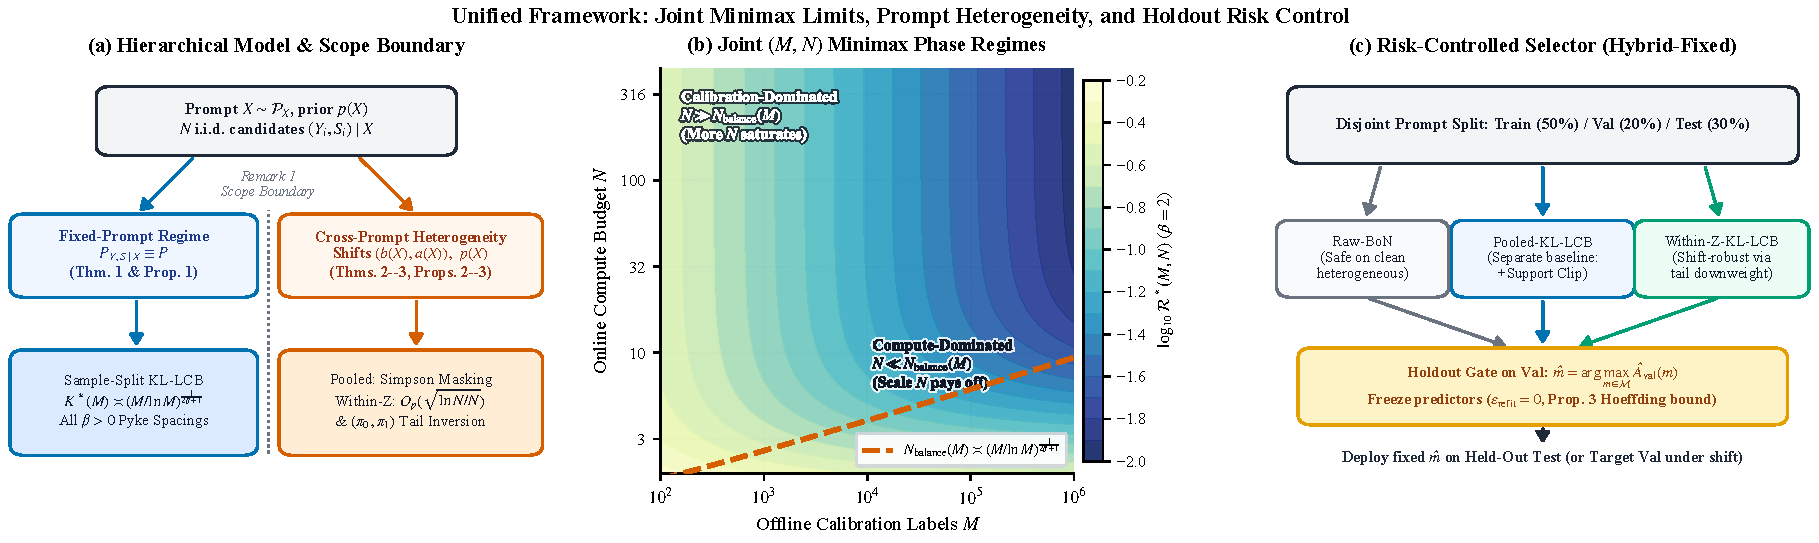
\includegraphics[width=0.78\textwidth]{fig1_framework_overview}
\caption{\textbf{Framework overview.} \textbf{(a)} Two-level prompt--candidate model separating single-prompt calibration ($P_{Y, S \mid X} \equiv P$, \Cref{sec:minimax}, and multi-verifier tails, \Cref{sec:ensemble}) from heterogeneous cross-prompt pooling ($X \sim \mathcal{P}_X$, \Cref{sec:heterogeneity}). \textbf{(b)} Theoretical joint $(M, N)$ minimax excess regret contour ($\beta=2$) and calibration--compute balance frontier $N_{\mathrm{balance}}(M) \asymp (M/\ln M)^{1/5}$ dividing compute-dominated ($N \ll N_{\mathrm{balance}}$) and calibration-dominated ($N \gg N_{\mathrm{balance}}$) regimes. \textbf{(c)} Minimal three-branch holdout gate ($\mathrm{Hybrid\text{-}Fixed}$, \Cref{alg:hybrid-fixed}) choosing among $\mathrm{Raw\text{-}BoN}$, $\mathrm{Pooled\text{-}KL\text{-}LCB}$, and $\mathrm{Within\text{-}Prompt\text{-}Z\text{-}KL\text{-}LCB}$ by validation accuracy.}
\label{fig:overview}
\end{figure}

Standard $\mathrm{BoN}$ draws uniformly from $\mathcal{I}_{\max} := \{i : S_i = S_{(N)}\}$ with accuracy $P_{\mathrm{BoN}}(N) := \Prob(Y_{i^*} = 1)$. For a fixed prompt $X=x$ (or homogeneous population $P_{Y, S \mid X} \equiv P$), dropping $X$ gives prior $p \in (0,1)$, mixture $\Fmix = p F_1 + (1-p)F_0$, $\barFmix = 1 - \Fmix$, and Radon--Nikodym posterior $q(s) = \frac{d(p\mu_1)}{d\mu_{\mathrm{mix}}}(s)$. Allowing countable tie atoms $\mathcal{A}$ and left-continuous quantile $\Fmix^{-1}(u) := \inf\{x : \Fmix(x) \ge u\}$, \Cref{thm:app-pit} (\Cref{app:preliminaries}) gives
\begin{equation}
\label{eq:pit-exact}
P_{\mathrm{BoN}}(N) = \int_{\R} q(x)\, d\big([\Fmix(x)]^N\big) = \int_0^1 q\big(\Fmix^{-1}(v^{1/N})\big)\, dv.
\end{equation}
Whenever $\lim_{x \uparrow x_R} f_1(x)/f_0(x) = 0$ (e.g., $\sigma_0 > \sigma_1$ or heavy wrong-tail spikes), $\lim_{N\to\infty} P_{\mathrm{BoN}}(N) = 0$ (\Cref{thm:app-collapse}), whereas exact posterior selection yields $P_{\mathrm{Cal\text{-}BoN}}(N) \uparrow \operatorname{ess\,sup} q(S)$ (\Cref{thm:app-cal}).

\paragraph{Estimation vs.\ Pooling Misspecification Decomposition.}
Consider any permutation-equivariant scoring rule $g_N : \R^N \to \R^N$ (covering shared scalar calibrators $g_N(S_{1:N})_i = \hat{g}(S_i)$ fitted on $\mathcal{D}_M$ toward a population target $g^*$, as well as prompt-wise normalizations such as sample Z-scores) that selects $\hat{i}_N(g_N) \sim \mathrm{Unif}(\arg\max_{1\le i\le N} g_N(S_{1:N})_i)$, with $\mathcal{D}_M$ independent of $(X, S_{1:N}, Y_{1:N})$. Relative to prompt-wise oracle posterior selection $\hat{i}_N^{\mathrm{oracle}} \in \arg\max_{1\le i\le N} q_X(S_i)$ and a population target rule $g_N^*$, the overall excess regret over $\mathcal{P}_X$ decomposes as
\begin{align}
\underbrace{\E\Big[\max_{1\le i\le N} q_X(S_i) - q_X\big(S_{\hat{i}_N(\hat{g}_N)}\big)\Big]}_{\text{Total heterogeneous excess regret}}
&= \underbrace{\E\Big[\max_{1\le i\le N} q_X(S_i) - q_X\big(S_{\hat{i}_N(g_N^*)}\big)\Big]}_{\text{Cross-prompt pooling misspecification (\Cref{sec:heterogeneity})}} \nonumber\\
&\quad + \underbrace{\E\Big[q_X\big(S_{\hat{i}_N(g_N^*)}\big) - q_X\big(S_{\hat{i}_N(\hat{g}_N)}\big)\Big]}_{\text{Finite-}(M,N)\text{ estimation discrepancy (\Cref{sec:minimax})}}.
\label{eq:regret-decomp}
\end{align}
Here the first term is always non-negative, whereas the second term can take either sign when $g_N^*$ is misspecified relative to $q_X$ and collapses to zero for deterministic prompt-wise rules ($g_N^* = \hat{g}_N$, such as \eqref{eq:sample-z}). When $P_{Y, S\mid X} \equiv P$ and $g_N^*(S_{1:N})_i = q(S_i)$, the first term vanishes and~\eqref{eq:regret-decomp} reduces to non-negative finite-$(M,N)$ excess regret relative to $q^*_P$ plus the irreducible $\Theta(N^{-\beta})$ oracle gap characterized in \Cref{thm:joint-minimax}.
\begin{remark}[Bridging Fixed-Prompt Minimax Theory and Heterogeneous Empirical Pooling]
\label{rem:scope}
Equation~\eqref{eq:regret-decomp} resolves the structural tension highlighted in \Cref{sec:intro} between single-distribution minimax rates (\Cref{sec:minimax}) and pooled multi-prompt experiments (\Cref{sec:experiments}). Conditioning on a single prompt or a homogeneous task ($P_{Y, S \mid X} \equiv P$) with target rule $g_N^*(S_{1:N})_i = q(S_i)$ sets the pooling misspecification term to zero, reducing~\eqref{eq:regret-decomp} entirely to non-negative finite-$(M, N)$ estimation regret relative to $q^*_P$ plus the irreducible $\Theta(N^{-\beta})$ oracle gap characterized in \Cref{thm:joint-minimax} (\Cref{sec:minimax}, plus \Cref{sec:ensemble} for fixed-prompt multi-RM tails). Under prompt heterogeneity, pooled estimation against $g^* = q_{\mathrm{pool}}$ still converges in finite-$(M, N)$ to its marginal target, yet the irreducible first term in~\eqref{eq:regret-decomp} can be strictly positive and even make $q_{\mathrm{pool}}$ perform worse than uncalibrated $\mathrm{Raw\text{-}BoN}$---precisely the Simpson confounding and Z-score inversion mechanisms analyzed in \Cref{sec:heterogeneity}.
\end{remark}

\section{Joint Calibration--Compute Minimax Theory}
\label{sec:minimax}

Fix $P$ (\Cref{rem:scope}) with passive offline labeled sample $\mathcal{D}_M = \{(\tilde{S}_j, \tilde{Y}_j)\}_{j=1}^M \sim P^{\otimes M}$ independent of online unlabeled scores $S_{1:N} \sim \Fmix^{\otimes N}$. Partitioning $\R$ into $K$ bins $\{B_k\}_{k=1}^K$ with masses $\pi_k = \Prob(S \in B_k) > 0$, bin posteriors $q_k = \Prob(Y=1 \mid S \in B_k)$, counts $m_k$, and successes $W_k$, any vector $\hat{\mathbf{s}} \in \R^K$ induces descending tie groups $G_1, \dots, G_L$ ($P_\ell = \sum_{k\in G_\ell}\pi_k$, $\bar{q}_\ell = P_\ell^{-1}\sum_{k\in G_\ell}\pi_k q_k$, $R_\ell = \sum_{j>\ell} P_j$) and exact conditional accuracy
\begin{equation}
\label{eq:cond-bin}
P(N \mid \mathcal{D}_M) = \sum_{\ell=1}^L \bar{q}_\ell\big[(R_\ell + P_\ell)^N - R_\ell^N\big], \qquad \lim_{N\to\infty} P(N \mid \mathcal{D}_M) = \bar{q}_1.
\end{equation}
Here~\eqref{eq:cond-bin} holds strictly when tied candidates in $\arg\max_i \hat{s}_{k(S_i)}$ are broken uniformly at random; breaking bin ties by continuous raw scores $S_i$ violates $\E[Y_{\hat{i}^*} \mid \mathcal{F}_{\mathrm{bins}}] = q_{\hat{k}^*}$ and restores within-bin tail collapse if a suboptimal high-score sub-region lies inside the top bin. Under empirical means $\hat{q}_k = W_k/m_k$ ($\mathrm{MLE}$), sparse inferior bins ($q_{k_0} < q^*$) hit $1$ with probability $(q_{k_0})^{m_{k_0}}$, pulling $\bar{q}_1$ down. Using binomial $\mathrm{KL\text{-}LCB}$ \citep{garivier2011kl} at level $\delta_{\mathrm{cov}} \in (0, 1)$ ($\hat{s}_k^{\mathrm{KL\text{-}LCB}} = 0$ if $m_k = 0$),
\begin{equation}
\label{eq:kl-lcb}
\hat{s}_k^{\mathrm{KL\text{-}LCB}}(\delta_{\mathrm{cov}}) := \inf\left\{q \in [0, \hat{q}_k] : m_k\, \KL(\hat{q}_k, q) \le \ln\frac{K}{\delta_{\mathrm{cov}}}\right\},
\end{equation}
guarantees $\hat{s}_k^{\mathrm{KL\text{-}LCB}} \le q_k$ simultaneously over all $k$ w.p.\ $\ge 1 - \delta_{\mathrm{cov}}$. By contrast, the finite-sample empirical Bernstein lower bound ($0$ if $m_k \le 1$, and for $m_k \ge 2$ with $\hat{v}_k := \frac{m_k}{m_k-1}\hat{q}_k(1-\hat{q}_k)$),
\begin{equation}
\label{eq:eb-lcb}
\hat{s}_k^{\mathrm{EB}}(\delta_{\mathrm{cov}}) := \left(\hat{q}_k - \sqrt{\frac{2\hat{v}_k \ln(2K/\delta_{\mathrm{cov}})}{m_k}} - \frac{7\ln(2K/\delta_{\mathrm{cov}})}{3(m_k - 1)}\right)_+,
\end{equation}
collapses deterministically to $0$ whenever $m_k < 1 + \frac{7}{3\hat{q}_k}\ln\frac{2K}{\delta_{\mathrm{cov}}}$.

\subsection{Uniformly Regular Peak Classes and Joint Minimax Bounds}

\begin{definition}[Pointwise Separated Class vs.\ Uniformly Regular Peak Class]
\label{def:classes}
Fix smoothness $\beta > 0$.
\begin{enumerate}[leftmargin=1.6em,itemsep=1pt,topsep=1pt]
    \item $P \in \mathcal{F}_\beta^{\mathrm{sep}}$ if $\Fmix$ is globally continuous with positive density $\fmix$, $f^* := \fmix(x^*) > 0$ at a unique maximizer $x^*$ of $q$, $q^* - q(x) = C|x - x^*|^\beta(1 + o(1))$ ($x \to x^*, C > 0$), and $\sup_{|x-x^*|\ge\eta} q(x) \le q^* - \varepsilon_\eta$ ($\forall\,\eta > 0$).
    \item Given $C_1, f_{\min}, \eta_0 > 0$ with $2\eta_0 f_{\min} < 1$, $P \in \mathcal{F}_\beta^{\mathrm{unif}}(C_1, f_{\min}, \eta_0)$ if $\Fmix$ is globally absolutely continuous on $\R$ with Radon--Nikodym density $\fmix$, $q^* := \sup_x q(x)$ is attained at some $x^* \in \R$, and on $U_{\eta_0} := [x^* - \eta_0, x^* + \eta_0]$,
    \begin{equation}
    \label{eq:unif-class}
    \fmix(x) \ge f_{\min} > 0 \qquad \text{and} \qquad q^* - q(x) \le C_1 |x - x^*|^\beta \qquad (\forall\, x \in U_{\eta_0}).
    \end{equation}
\end{enumerate}
\end{definition}

\begin{remark}[Necessity of Class Constants Without Uniform Global Separation]
\label{rem:constants}
Without uniform curvature $C_1$ in~\eqref{eq:unif-class}, even an exact oracle suffers $\Theta(1)$ minimax regret: $S \sim \mathcal{N}(0, 1)$, $q_h(s) = \frac{1}{4} + \frac{1}{2}e^{-s^2/h^2}$ gives $q_h^* - \E[\max_{i\le N} q_h(S_i)] \ge \frac{1}{2} - \frac{Nh}{2\sqrt{h^2+2}} \to \frac{1}{2}$ as $h \downarrow 0$. Conversely, a uniform global separation gap would exclude the shrinking Fano bumps needed for lower bounds.
\end{remark}

\begin{theorem}[Joint Calibration--Compute Minimax Limits and Balance Law]
\label{thm:joint-minimax}
Under \Cref{def:classes}, let $\beta > 0$ and $c_\beta := \max(1, 2^{\beta-1})$.
\begin{enumerate}[leftmargin=1.6em,itemsep=2pt,topsep=1pt]
    \item \textbf{(Pointwise Oracle Rate)} For any fixed $P \in \mathcal{F}_\beta^{\mathrm{sep}}$, exact posterior $\mathrm{BoN}$ ($M = \infty$) satisfies $q^*_P - P_{\mathrm{Cal\text{-}BoN}}(N) = \big(1 + o(1)\big)\,\frac{\Gamma(\beta + 1)\,C}{(2 f^*)^\beta}\,N^{-\beta}$.
    \item \textbf{(Uniform Upper Bound)} On $\mathcal{F}_\beta^{\mathrm{unif}}(C_1, f_{\min}, \eta_0)$, fix any positive bin-schedule prefactor $c_0 > 0$ (whose rate-optimal choice scales with $(C_1, f_{\min})$) and let equal-frequency bins ($\pi_k = 1/K$) use $K = K^*(M) := \lfloor c_0 (M/\ln M)^{\frac{1}{2\beta+1}}\rfloor$ with $\delta_{\mathrm{cov}} = \frac{1}{3M}$ in~\eqref{eq:kl-lcb}. For every $(M, N)$ with $N \ge 1$ and $M$ satisfying $K > \frac{2}{\eta_0 f_{\min}}$ and $M \ge 8 K \ln(3KM)$,
    \begin{multline}
    \label{eq:joint-upper}
    \sup_{P \in \mathcal{F}_\beta^{\mathrm{unif}}}\Big(q^*_P - \E_{\mathcal{D}_M}\big[P_{\mathrm{KL\text{-}LCB}}(N \mid \mathcal{D}_M)\big]\Big)
    \le \frac{1}{M} + e^{-\eta_0 f_{\min} N} + \frac{C_1 c_\beta}{(K f_{\min})^\beta} \\
    + 2\sqrt{\frac{K\ln(3KM)}{M}} + \frac{C_1 c_\beta \Gamma(\beta+1)}{(2 f_{\min})^\beta}N^{-\beta}.
    \end{multline}
    \item \textbf{(All-Policy Lower Bound and Balance Law)} When the support contains an interval of positive Lebesgue measure carrying density $\ge f_{\min}$ that admits disjoint bump perturbations and a member $P^* \in \mathcal{F}_\beta^{\mathrm{unif}} \cap \mathcal{F}_\beta^{\mathrm{sep}}$, then for all sufficiently large $M$ and all $N \ge 1$, over all measurable policies $\pi(\mathcal{D}_M, S_{1:N}) \in \{1,\dots,N\}$,
    \begin{equation}
    \label{eq:joint-lower}
    \inf_{\pi}\ \sup_{P \in \mathcal{F}_\beta^{\mathrm{unif}}}\Big(q^*_P - \E_{P^{\otimes(M+N)}}\big[q_P(S_{\pi(\mathcal{D}_M, S_{1:N})})\big]\Big)
    = \Omega\!\left(\left(\frac{\ln M}{M}\right)^{\frac{\beta}{2\beta+1}} + N^{-\beta}\right).
    \end{equation}
    Equating~\eqref{eq:joint-upper} and~\eqref{eq:joint-lower} gives the \emph{calibration--compute balance threshold}
    \begin{equation}
    \label{eq:n-balance}
    N_{\mathrm{balance}}(M) \asymp \left(\frac{M}{\ln M}\right)^{\frac{1}{2\beta+1}} \asymp K^*(M) \qquad \Big(\beta=2:\ \Big(\frac{M}{\ln M}\Big)^{1/5}\Big),
    \end{equation}
    separating online-compute-dominated ($N \ll N_{\mathrm{balance}}$) from calibration-dominated ($N \gg N_{\mathrm{balance}}$) scaling (\Cref{fig:overview}(b); see \Cref{rem:constants} on $C_1$).
\end{enumerate}
\end{theorem}

\subsection{Unknown Marginals: All-\texorpdfstring{$\beta$}{beta} Sample-Split Spacings and Algorithm}

When $\Fmix$ is unknown with no external unlabeled pool, additive DKW bounds yield relative bin-mass error $K^*(M)\sqrt{(\ln M)/M} \asymp (M/\ln M)^{\frac{1-2\beta}{2(2\beta+1)}}$, which fails to vanish for $0 < \beta \le 1/2$. \Cref{alg:split-kl-lcb} covers all $\beta > 0$ via sample-split Pyke spacings (\Cref{app:minimax}).

\begin{algorithm}[htbp]
\caption{Sample-Split Equal-Frequency $\mathrm{KL\text{-}LCB}$ (with Optional Support Clipping)}
\label{alg:split-kl-lcb}
\DontPrintSemicolon
\KwIn{Offline pairs $\mathcal{D}_M = \{(\tilde{S}_j, \tilde{Y}_j)\}_{j=1}^M$, smoothness $\beta > 0$, prefactor $c_0 > 0$, $\delta_{\mathrm{cov}} \in (0,1)$, test scores $S_{1:N}$, clip quantile $\tau_{\mathrm{clip}} \in (0, 1]$ (default $1$)}
\KwOut{Selected candidate index $\hat{i}^* \in \{1, \dots, N\}$}
Split $\mathcal{D}_M = \mathcal{D}_{M_1}^{\mathrm{edge}} \sqcup \mathcal{D}_{M_2}^{\mathrm{est}}$ ($M_1 = \lfloor M/2\rfloor$); set $K \leftarrow \min\big(M_1 + 1,\, \max\big(2, \lfloor c_0 (M/\ln M)^{\frac{1}{2\beta+1}}\rfloor\big)\big)$.\;
Sort $\mathcal{D}_{M_1}^{\mathrm{edge}}$ as $S_{(1)}^{\mathrm{edge}} \le \dots \le S_{(M_1)}^{\mathrm{edge}}$; set $r_0 = 0$, $r_k = \lfloor \frac{k(M_1+1)}{K}\rfloor$ ($1 \le k < K$), $r_K = M_1 + 1$, $\hat{e}_k = S_{(r_k)}^{\mathrm{edge}}$ ($1 \le k < K$), $\hat{e}_0=-\infty, \hat{e}_K=+\infty$, $s_{\max} = S_{(\lceil \tau_{\mathrm{clip}} M_1\rceil)}^{\mathrm{edge}}$.\;
\For{$k = 1, \dots, K$}{
    Count $m_k, W_k$ on $\mathcal{D}_{M_2}^{\mathrm{est}}$ inside $(\hat{e}_{k-1}, \hat{e}_k]$; compute $\hat{s}_k \leftarrow \hat{s}_k^{\mathrm{KL\text{-}LCB}}(\delta_{\mathrm{cov}})$ via~\eqref{eq:kl-lcb} ($0$ if $m_k=0$).\;
}
For each $i \in \{1,\dots,N\}$, assign $\hat{v}_i \leftarrow \hat{s}_{k(S_i)}$ if ($\tau_{\mathrm{clip}} = 1$ or $S_i \le s_{\max}$), else $\hat{v}_i \leftarrow -1$ (strictly below all $\hat{s}_k \ge 0$).\;
\Return{$\hat{i}^* \sim \mathrm{Unif}\big(\arg\max_{1\le i\le N} \hat{v}_i\big)$ (strictly uniform random tie-breaking so $\E[Y_{\hat{i}^*} \mid \mathcal{F}_{\mathrm{bins}}] = q_{\hat{k}^*}$).}
\end{algorithm}

\begin{proposition}[Sample-Split Quantile Spacings for All $\beta > 0$]
\label{prop:spacings}
Under continuous $\Fmix$, execute \Cref{alg:split-kl-lcb} with $\delta_{\mathrm{cov}} = \frac{1}{4M}$ and $\tau_{\mathrm{clip}} = 1$. Whenever $M_1 + 1 \ge \max(12 K,\, 214\ln(16M))$ and $d_{\min} := \min_{1\le k\le K}(r_k - r_{k-1}) \ge 9.1\ln(16KM)$ (which holds for $K^*(M)$ across every $\beta > 0$ at large $M$), w.p.\ $\ge 1 - \frac{1}{4M}$ simultaneously for all $1 \le k \le K$, $\frac{1}{2K} \le \hat{\pi}_k := \Fmix(\hat{e}_k) - \Fmix(\hat{e}_{k-1}) \le \frac{143}{72 K} < \frac{2}{K}$. If additionally $M_2 \ge 16 K\ln(4KM)$ and $K > \frac{4}{\eta_0 f_{\min}}$, then on $\mathcal{F}_\beta^{\mathrm{unif}}$,
\begin{multline}
q^*_P - \E_{\mathcal{D}_M}\big[P_{\mathrm{Split\text{-}KL\text{-}LCB}}(N \mid \mathcal{D}_M)\big]
\le \frac{1}{M} + e^{-\eta_0 f_{\min} N} + \frac{2^\beta C_1 c_\beta}{(K f_{\min})^\beta} \\
+ 4\sqrt{\frac{K\ln(4KM)}{M}} + \frac{C_1 c_\beta\Gamma(\beta+1)}{(2 f_{\min})^\beta}N^{-\beta},
\end{multline}
inflating the bin bias bound by at most $2^\beta$ and the leading statistical confidence coefficient from $2$ to $4$ (a factor of $2$, up to replacing $\ln(3KM)$ by $\ln(4KM)$ inside the radical) vs.~\eqref{eq:joint-upper} using zero external unlabeled samples; \eqref{eq:eb-lcb} still collapses when $m_k$ falls below its linear threshold.
\end{proposition}

\section{Prompt Heterogeneity, Sample Standardization, and Risk Control}
\label{sec:heterogeneity}

Returning to $X \sim \mathcal{P}_X$ (\Cref{sec:model,rem:scope}), let $q_X(s) = \Prob(Y=1 \mid S=s, X)$ and $q_{\mathrm{pool}}(s) = \Prob(Y=1 \mid S=s)$ (proofs in \Cref{app:heterogeneity}).

\subsection{Simpson Derivative Decomposition and Grid-Free Masking}

\begin{theorem}[Simpson Posterior Decomposition and Grid-Free Analytical Masking]
\label{thm:simpson}
For $C^1$ strictly positive $f_{c, X}(s)$ with $g_X(s) := \partial_s \ln f_{\mathrm{mix}, X}(s)$ satisfying differentiation under the integral sign: (1) $q'_{\mathrm{pool}}(s) = \E[\partial_s q_X(s) \mid S = s] + \Cov(Y,\, g_X(s) \mid S = s)$ for all $s \in \R$; and (2) under two Gaussian strata with $(w_1, w_2) = (0.85, 0.15)$, $(p_1, p_2) = (0.05, 0.95)$, shifts $(b_1, b_2) = (0.0, 3.0)$, and base $(\mu_{1,\mathrm{base}}, \mu_{0,\mathrm{base}}, \sigma_1, \sigma_0) = (0.3, 0.0, 1.0, 2.0)$, analytically at every point $s \in [3.5, 4.2]$,
\begin{equation}
\partial_s q_1(s) < -1.10\times 10^{-3} < 0, \quad \partial_s q_2(s) < -1.85\times 10^{-3} < 0, \quad q'_{\mathrm{pool}}(s) > +7.03\times 10^{-3} > 0
\end{equation}
(precisely $> +7.044\times 10^{-3}$), masking strict collapse inside both strata with positive pooled slope.
\end{theorem}

\subsection{Within-Prompt Z-Scores: \texorpdfstring{$N=2$}{N=2} Rank Ceiling and General-\texorpdfstring{$(\pi_0,\pi_1)$}{(pi0, pi1)} Tail Inversion}

Suppose $S_i = b(X) + a(X)\tilde{S}_i$ ($a(X) > 0$) where the base scores follow prompt-invariant class-conditional laws $\tilde{S}_i \mid (Y_i = c, X) \sim \tilde{F}_c$ ($c \in \{0, 1\}$) with prompt-dependent mixture moments $(\tilde{\mu}(X), \tilde{\sigma}^2(X))$ and posterior $\tilde{q}_X(\tilde{s}) \equiv q_X(b(X) + a(X)\tilde{s})$ (into which heterogeneous prior $p(X)$ enters). For $N \ge 2$ candidates per prompt, with $\bar{S}_N = \frac{1}{N}\sum_{i=1}^N S_i$ and $\hat{s}_N = \sqrt{\frac{1}{N-1}\sum_{i=1}^N(S_i - \bar{S}_N)^2}$, define the online sample Z-score
\begin{equation}
\label{eq:sample-z}
Z_{i, N} := \frac{S_i - \bar{S}_N}{\hat{s}_N} \ \ (\text{if }\hat{s}_N > 0), \qquad \text{and}\quad Z_{i,N} := 0 \ \ (\text{if }\hat{s}_N = 0).
\end{equation}

\begin{proposition}[Non-Degenerate Sample Z-Scores and Tight $N=2$ Rank Ceiling]
\label{prop:zscore-n2}
Assume $\E[\tilde{S}^4 \mid X] < \infty$ and $\tilde{\sigma}^2(X) > 0$ ($\mathcal{P}_X$-a.s.). (1) For $\mathcal{P}_X$-a.e.\ $X$ and \textbf{each fixed candidate index} $i \ge 1$ as $N \to \infty$, $\Prob(\hat{s}_N = 0 \mid X) \to 0$ and $Z_{i,N} \xrightarrow{\mathrm{a.s.}} Z_i^*(X) := \frac{\tilde{S}_i - \tilde{\mu}(X)}{\tilde{\sigma}(X)}$ at $O_p(N^{-1/2})$, canceling $(b(X), a(X))$ while leaving $(\tilde{\mu}(X), \tilde{\sigma}(X))$ drift from heterogeneous $p(X)$ (so even under prompt-invariant class laws $\tilde{F}_c$, the Z-standardized conditional distributions align across prompts only when $(\tilde{\mu}(X), \tilde{\sigma}(X))$ does not vary with $p(X)$). (2) At $N = 2$, $(Z_{1,2}, Z_{2,2}) \in \{(\pm 1/\sqrt{2}, \mp 1/\sqrt{2})\} \cup \{(0, 0)\}$; under uniform tie-breaking whenever $S_1 = S_2$ (continuous $F_{\mathrm{mix}, X}$ gives tie probability zero and $P_{\mathrm{Anti\text{-}BoN}}(2) = 2\bar{p} - P_{\mathrm{Raw}}(2)$), every $Z_{i,2}$-based rule obeys $P_{\mathrm{Within\text{-}Z}}(2) \le \max\big(P_{\mathrm{Raw}}(2),\, P_{\mathrm{Anti\text{-}BoN}}(2),\, \bar{p}\big) \le P_{\mathrm{Cal\text{-}BoN}}^{\mathrm{oracle}}(2)$. Equality with the oracle holds when $q_X$ is $\mathcal{P}_X$-a.s.\ non-decreasing (e.g., homoscedastic $\mathcal{N}(1,1)/\mathcal{N}(0,1), p=0.5$ yields $0.630125$) or $\mathcal{P}_X$-a.s.\ non-increasing, and under continuous $F_{\mathrm{mix},X}$ strict suboptimality holds \emph{iff} both $\{S_1 < S_2, q_X(S_1) > q_X(S_2)\}$ and $\{S_1 < S_2, q_X(S_1) < q_X(S_2)\}$ have positive probability.
\end{proposition}

Now consider general boundary prompt fractions: unsolvable prompts $\pi_0 := \Prob(p(X) = 0) \ge 0$, trivial prompts $\pi_1 := \Prob(p(X) = 1) \ge 0$ ($\pi_0 + \pi_1 > 0$), and positive mass $1 - \pi_0 - \pi_1 > 0$ of interior solvable prompts on $[p_{\min}, p_{\max}] \subset (0, 1)$, under a homoscedastic Gaussian verifier $\tilde{S}_i \mid (Y_i = c, X) \sim \mathcal{N}(\mu_c, \sigma^2)$ ($\Delta := \mu_1 - \mu_0 > 0$). Positive interior mass is necessary since purely two-point tasks $p(X) \in \{0, 1\}$ trivially attain $1 - \pi_0$ under any ranking. Real LLM benchmarks typically have $\pi_1 > 0$ alongside $\pi_0 > 0$ (\Cref{sec:experiments}), making a general-$(\pi_0, \pi_1)$ characterization essential.

\begin{theorem}[General-$(\pi_0, \pi_1)$ Tail Inversion and Online Sample-$Z_{i,N}$ Ceiling Loss]
\label{thm:sample-z-ceiling}
Let $q_{\mathrm{pool}, Z^*}(z) := \Prob(Y = 1 \mid Z^* = z)$, $\tilde{q}_X(\tilde{s}) := \Prob(Y=1 \mid \tilde{S}=\tilde{s}, X)$, and define the boundary tail ratio $L_{\mathrm{tail}} := \frac{\pi_1}{\pi_0 + \pi_1}$.
\begin{enumerate}[leftmargin=1.6em,itemsep=2pt,topsep=1pt]
    \item \textbf{(Unconditional Two-Sided Tail Limit and Regime Split)} Because $v(p) := \frac{\sigma^2}{\sigma^2 + p(1-p)\Delta^2} = 1$ at $p \in \{0, 1\}$ whereas $v(p) \le v_{\max} < 1$ on $[p_{\min}, p_{\max}]$, $\lim_{z \to \pm\infty} q_{\mathrm{pool}, Z^*}(z) = L_{\mathrm{tail}} = \frac{\pi_1}{\pi_0 + \pi_1}$.
    \begin{itemize}[leftmargin=1.2em,itemsep=1pt,topsep=1pt]
        \item[(a)] \emph{Unsolvable-free boundary regime ($\pi_0 = 0, \pi_1 > 0$):} Here $L_{\mathrm{tail}} = 1 > q_{\mathrm{pool}, Z^*}(z)$ for every $z \in \R$, so no compact global maximizer exists. Because both $z \to +\infty$ and $z \to -\infty$ converge to $1$, unconstrained two-sided maximization can suffer a \emph{left-tail overtake trap} when heterogeneous interior priors have large $\Delta/\sigma$, selecting $Z_{i,N} \to -\infty$ and driving interior prompt accuracy toward $0$. Under right-half ($z \ge 0$) constrained maximization $\hat{i}_N^{\ge 0} \in \arg\max_{i : Z_{i,N} \ge 0} q_{\mathrm{pool}, Z^*}(Z_{i,N})$ (which is always non-empty since $\sum_{i=1}^N Z_{i,N} = 0$), every prompt selects $Z_{\hat{i}_N^{\ge 0}}^*(X) \xrightarrow{p} +\infty$ and achieves $\lim_{N\to\infty} P_{\mathrm{Sample\text{-}Z\text{-}Cal}}^{\mathrm{right\text{-}half}}(N) = 1 = P_{\mathrm{Raw}}(\infty)$.
        \item[(b)] \emph{General unsolvable coexistence regime ($\pi_0 > 0, \pi_1 \ge 0$, $1-\pi_0-\pi_1 > 0$):} Since $\tilde{q}_X(\tilde{\mu}(X) + \tilde{\sigma}(X)z) \to 1 > L_{\mathrm{tail}}$ for interior strata, there always exists $z_0 \in \R$ with $q_{\mathrm{pool}, Z^*}(z_0) > L_{\mathrm{tail}}$; hence $K^* := \arg\max_{z \in \R} q_{\mathrm{pool}, Z^*}(z) \subset [-M_Z, M_Z]$ is non-empty and compact for \emph{all} $\pi_1 \ge 0$ (even if the global variance ratio satisfies $\kappa_Z < 1$, e.g., $\pi_0=0.01, \pi_1=0, p_1=0.1, p_2=0.2, \Delta=100, \sigma=1$ giving $\kappa_Z \approx 0.3103$).
    \end{itemize}
    \item \textbf{(Online Sample-$Z_{i,N}$ Convergence and Affine-Invariant Ceiling Loss)} Whenever $\pi_0 > 0, \pi_1 \ge 0$ with $1 - \pi_0 - \pi_1 > 0$ interior solvable mass (so $K^*$ is compact), online selection $\hat{i}_N \in \arg\max_{1\le i\le N} q_{\mathrm{pool}, Z^*}(Z_{i,N})$ via~\eqref{eq:sample-z} satisfies $\Delta_N(x) := \max_{1 \le i \le N} |Z_{i,N} - Z_i^*(x)| = O_p(\sqrt{(\ln N)/N}) \xrightarrow{p} 0$ for every $X = x$, and for arbitrary $(b(X), a(X) > 0)$,
    \begin{align}
    \limsup_{N \to \infty} P_{\mathrm{Sample\text{-}Z\text{-}Cal}}^{\mathrm{oracle}}(N)
    &\le \pi_1 + \E_X\!\left[\max_{z \in K^*} q_X\!\big(b(X) + a(X)[\tilde{\mu}(X) + \tilde{\sigma}(X)z]\big)\,\ind\{p(X)\in(0,1)\}\right] \nonumber\\
    &\equiv \pi_1 + \E_X\!\left[\max_{z \in K^*} \tilde{q}_X\!\big(\tilde{\mu}(X) + \tilde{\sigma}(X)z\big)\,\ind\{p(X)\in(0,1)\}\right] < 1 - \pi_0 = P_{\mathrm{Raw}}(\infty).
    \end{align}
    \emph{Finite-budget mitigation:} as $\pi_1/\pi_0$ increases, $K^*$ shifts toward extreme right-tail quantiles ($z \gg 1$) and the asymptotic gap $P_{\mathrm{Raw}}(\infty) - P_{\mathrm{Sample\text{-}Z\text{-}Cal}}^{\mathrm{oracle}}(\infty)$ shrinks; qualitatively, this right-tail shift trend persists even under skewed or multimodal real score distributions, explaining why benchmarks with large $\hat{\pi}_1$ exhibit milder finite-$N$ Z-score drops than $\hat{\pi}_0$-heavy benchmarks.
\end{enumerate}
\end{theorem}

\subsection{Minimal Holdout Risk-Control Baseline}

Because no fixed scoring rule dominates across all regimes (\Cref{thm:simpson,prop:zscore-n2,thm:sample-z-ceiling}), \Cref{alg:hybrid-fixed} presents a minimal three-branch validation selector ($\mathrm{Hybrid\text{-}Fixed}$) as a risk-control baseline rather than a new learning algorithm. The outlier-filtering baseline $\mathrm{Support\text{-}Clipped}$ ($\tau_{\mathrm{clip}} < 1$ in \Cref{alg:split-kl-lcb}) is audited separately in \Cref{sec:experiments} and is deliberately excluded from the candidate family $\mathcal{M}$ below.

\begin{algorithm}[htbp]
\caption{Minimal Three-Branch Holdout Risk-Control Baseline ($\mathrm{Hybrid\text{-}Fixed}$ vs.\ $\mathrm{Hybrid\text{-}Refit}$)}
\label{alg:hybrid-fixed}
\DontPrintSemicolon
\KwIn{Disjoint prompt split $\mathcal{D}_{\mathrm{train}} \sqcup \mathcal{D}_{\mathrm{val}} \sqcup \mathcal{D}_{\mathrm{test}}$, budget $N \ge 2$, mode $\in \{\mathrm{Fixed}, \mathrm{Refit}\}$}
\KwOut{Selected branch $\hat{m}$ and held-out accuracies}
Fit $\mathrm{Pooled\text{-}KL\text{-}LCB}$ and $\mathrm{Within\text{-}Prompt\text{-}Z\text{-}KL\text{-}LCB}$ (via~\eqref{eq:sample-z}) on $\mathcal{D}_{\mathrm{train}}$, forming $\mathcal{M}$ ($|\mathcal{M}| = 3$) with $\mathrm{Standard\text{-}BoN}$.\;
Evaluate $\hat{A}_{\mathrm{val}}(m)$ at budget $N$ on $\mathcal{D}_{\mathrm{val}}$ and select $\hat{m} \in \arg\max_{m \in \mathcal{M}} \hat{A}_{\mathrm{val}}(m)$.\;
\lIf{$\mathrm{mode} = \mathrm{Fixed}$}{deploy frozen $\mathcal{D}_{\mathrm{train}}$-fitted $\hat{m}$ on $\mathcal{D}_{\mathrm{test}}$ ($\varepsilon_{\mathrm{refit}} \equiv 0$).}
\lElse{refit $\hat{m}$ on $\mathcal{D}_{\mathrm{train}} \cup \mathcal{D}_{\mathrm{val}}$ before testing on $\mathcal{D}_{\mathrm{test}}$.}
\end{algorithm}

\begin{proposition}[Holdout Risk-Control Bound and Refit Stability]
\label{prop:hybrid}
For any $N \ge 2$, assume $\mathcal{D}_{\mathrm{val}}$ comprises $M_{\mathrm{val}} = |\mathcal{D}_{\mathrm{val}}|$ i.i.d.\ prompts drawn from the deployment distribution and independent of $\mathcal{D}_{\mathrm{train}}$. Conditional on $\mathcal{D}_{\mathrm{train}}$, \Cref{alg:hybrid-fixed} guarantees: (1) under $\mathrm{Hybrid\text{-}Fixed}$, $\max_{m\in\mathcal{M}} A_{\mathrm{fixed}}(m) - A_{\mathrm{fixed}}(\hat{m}) \le 2\sqrt{\frac{\ln(2|\mathcal{M}|/\delta)}{2 M_{\mathrm{val}}}}$ w.p.\ $\ge 1 - \delta$, and in expectation over $\mathcal{D}_{\mathrm{val}}$, $\max_{m\in\mathcal{M}} A_{\mathrm{fixed}}(m) - \E_{\mathrm{val}}[A_{\mathrm{fixed}}(\hat{m})] \le \sqrt{\frac{\ln|\mathcal{M}|}{2 M_{\mathrm{val}}}}$; and (2) under $\mathrm{Hybrid\text{-}Refit}$ with (in general random) refit shift modulus $\varepsilon_{\mathrm{refit}} := \max_{m\in\mathcal{M}}|A_{\mathrm{refit}}(m) - A_{\mathrm{fixed}}(m)|$ conditional on $(\mathcal{D}_{\mathrm{train}}, \mathcal{D}_{\mathrm{val}})$, $\max_{m\in\mathcal{M}} A_{\mathrm{refit}}(m) - A_{\mathrm{refit}}(\hat{m}) \le 2\sqrt{\frac{\ln(2|\mathcal{M}|/\delta)}{2 M_{\mathrm{val}}}} + 2\varepsilon_{\mathrm{refit}}$ w.p.\ $\ge 1 - \delta$ (while under train--test distribution shift, validation regret controls only target-matched shifts unless $\mathcal{D}_{\mathrm{val}}$ is drawn from the target domain).
\end{proposition}

\section{Supplementary Structural Analysis: Multi-Verifier Tail Dependence}
\label{sec:ensemble}

For completeness under a fixed prompt (\Cref{rem:scope}), we summarize when $K \ge 2$ verifiers $\mathbf{S} \in \R^K$ can reverse tail collapse via correlation asymmetry \citep{coste2024reward,rame2024warm} (\Cref{app:ensemble,fig:multi-rm}). As \Cref{sec:experiments} shows, enforcing asymptotic tail safety constraints incurs a conservative accuracy tax on low-$N$, non-collapsing pools.

\begin{theorem}[Gaussian Spectral Path with Orthogonal Boundary, Weakly Active $\mathrm{Min}$, and QDA]
\label{thm:gaussian-ensemble}
Let $\mathbf{S} \mid (Y = c) \sim \mathcal{N}(\boldsymbol{\mu}_c, \Sigma_c)$ ($\Sigma_c \succ 0$) with $\Delta\boldsymbol{\mu} := \boldsymbol{\mu}_1 - \boldsymbol{\mu}_0 \neq \mathbf{0}$. Perform simultaneous congruence $P^\top\Sigma_1 P = I_K$ and $P^\top\Sigma_0 P = \operatorname{diag}(\lambda_1,\dots,\lambda_K)$ ($0 < \lambda_1 \le \dots \le \lambda_K$, $\lambda_{\min} = \lambda_1$), writing $\mathbf{d} := P^\top\Delta\boldsymbol{\mu}$, $\mathbf{v} := P^{-1}\mathbf{w}$, $I_{\min} := \{k : \lambda_k = \lambda_{\min}\}$, $V_{\min} := \operatorname{span}\{\mathbf{e}_k : k \in I_{\min}\}$, and $P_{V_{\min}}$ for the Euclidean orthogonal projection onto $V_{\min}$.
\begin{enumerate}[leftmargin=1.6em,itemsep=2pt,topsep=1pt]
    \item \textbf{(Linear Reversal and Complete $N=2$ $\mathrm{Safe\text{-}Fisher}$ Solution)} A direction $\mathbf{w} \neq \mathbf{0}$ achieves $\lim_{N\to\infty}\allowbreak P_{\mathrm{BoN}}(N;\allowbreak \mathbf{w}^\top\mathbf{S}) = 1$ iff $\lambda_{\min} < 1$ (or $\lambda_{\min} = 1$ with $\mathbf{w}^{*\top}\Delta\boldsymbol{\mu} > 0$ for some $\lambda_{\min}$-eigenvector $\mathbf{w}^*$). For symmetric equal-variance $2$-verifier pairs with class-$c$ off-diagonal correlation $\rho_c$ ($\sigma_{0,k} = \kappa\sigma_{1,k}$, $\kappa > 1$), difference fusion cancels shared wrong-answer variance whenever $\rho_0 > \rho_1$ satisfies $\kappa^2\frac{1-\rho_0}{1-\rho_1} < 1$. Maximizing $\SNR_2^2(\mathbf{w}) = \frac{(\mathbf{w}^\top\Delta\boldsymbol{\mu})^2}{\mathbf{w}^\top(\Sigma_1+\Sigma_0)\mathbf{w}}$ s.t.\ $R(\mathbf{w}) := \frac{\mathbf{w}^\top\Sigma_0\mathbf{w}}{\mathbf{w}^\top\Sigma_1\mathbf{w}} \le \kappa_{\max}^2$ under Slater feasibility $\lambda_{\min} < \kappa_{\max}^2 < R(\mathbf{w}_{\mathrm{Fisher}})$ (where $\mathbf{w}_{\mathrm{Fisher}} := (\Sigma_1 + \Sigma_0)^{-1}\Delta\boldsymbol{\mu}$ maximizes $\SNR_2^2$) exhibits two exact branches via $x_k = v_k^2$ convexification: \emph{(a) Interior branch:} if $P_{V_{\min}}\mathbf{d} \neq \mathbf{0}$ (or $P_{V_{\min}}\mathbf{d} = \mathbf{0}$ with $\lim_{\tau \uparrow \lambda_{\min}^-} R(\mathbf{w}_\tau) < \kappa_{\max}^2$), the optimum lies on $\mathbf{w}_\tau = (\Sigma_0 - \tau\Sigma_1)^{-1}\Delta\boldsymbol{\mu}$ ($\tau \in [-1, \lambda_{\min})$, $R(\mathbf{w}_{\tau^*}) = \kappa_{\max}^2$, targeted at $N=2$); \emph{(b) Degenerate orthogonal branch:} if $P_{V_{\min}}\mathbf{d} = \mathbf{0}$ and $\lim_{\tau \uparrow \lambda_{\min}^-} R(\mathbf{w}_\tau) \ge \kappa_{\max}^2$ (e.g., $\Sigma_1 = I_2, \Sigma_0 = \operatorname{diag}(0.5, 2.0), \Delta\boldsymbol{\mu} = (0,1)^\top, \kappa_{\max}^2 = 1$), $\mathbf{w}_\tau$ stays outside the constraint and the optimum saturates at $\tau^* = \lambda_{\min}$ via orthogonal mixing $\mathbf{w}^* = \mathbf{w}_{\lambda_{\min}^-} + \alpha\mathbf{u}_{\min}$ ($\mathbf{u}_{\min} \in P V_{\min}\setminus\{\mathbf{0}\}$, $\mathbf{u}_{\min}^\top \Sigma_1 \mathbf{u}_{\min} = 1$, $R(\mathbf{w}^*) = \kappa_{\max}^2$, giving $\mathbf{w}^* \propto (\sqrt{2}, 1)^\top$). When $\Sigma_0 \succ \Sigma_1$ ($\lambda_{\min} > 1$), the Bayes QDA posterior satisfies $q^*_{\mathrm{Bayes}} := \sup_{\mathbf{s}} q_{\mathrm{Bayes}}(\mathbf{s}) < 1$ and converges to $q^*_{\mathrm{Bayes}}$ at rate $\Theta(N^{-2/K})$.
    \item \textbf{($\mathrm{Min\text{-}Ensemble}$ with Zero-Multiplier Active Sets)} For $M_{\min}(\mathbf{S}) = \min_{1\le k\le K} S^{(k)}$, let $\mathbf{u}_c^* = \arg\min_{\mathbf{u}\ge\mathbf{1}_K}\mathbf{u}^\top\Sigma_c^{-1}\mathbf{u}$ with value $\gamma_c > 0$ and KKT multipliers $\mathbf{w}_c = \Sigma_c^{-1}\mathbf{u}_c^* \ge \mathbf{0}$ \citep{savage1962mills,hashorva2003multivariate}. Partition $\{1,\dots,K\}$ into essential active $I_{+,c} = \{k : w_{c,k} > 0\}$, weakly active $I_{0,c} = \{k : u_{c,k}^*=1, w_{c,k}=0\}$, and strictly inactive $J_c = \{k : u_{c,k}^* > 1\}$. Let $\beta_c := \mathbf{w}_{c, I_{+,c}}^\top \boldsymbol{\mu}_{c, I_{+,c}}$ and let $\theta_{c, I_0} := \Prob(\mathbf{W}_{I_{0,c}} > \mathbf{0}) \in (0, 1]$ ($1$ if $I_{0,c}=\emptyset$) denote the positive-orthant survival probability of the Schur-complement Gaussian vector $\mathbf{W}_{I_{0,c}} \sim \mathcal{N}(\tilde{\boldsymbol{\mu}}_{0|+},\allowbreak\,\tilde{\Sigma}_{0|+})$, and define the scale prefactor $C_c^{\mathrm{sf}} > 0$ by
    \[
    C_c^{\mathrm{sf}} := \theta_{c, I_0}(2\pi)^{-|I_{+,c}|/2}(\det \Sigma_{c, I_{+,c}I_{+,c}})^{-1/2}\Big(\prod_{k\in I_{+,c}} w_{c,k}^{-1}\Big)\exp\!\Big(-\tfrac{1}{2}\boldsymbol{\mu}_{c, I_{+,c}}^\top\Sigma_{c, I_{+,c}I_{+,c}}^{-1}\boldsymbol{\mu}_{c, I_{+,c}}\Big) > 0.
    \]
    As $t \to +\infty$, $f_{\min, c}(t) = \big(1 + o(1)\big)\, \gamma_c C_c^{\mathrm{sf}}\, t^{1 - |I_{+,c}|}\exp\!\left(-\frac{\gamma_c}{2}t^2 + \beta_c t\right)$, governed by $|I_{+,c}|$ rather than $|I_{+,c} \cup I_{0,c}|$.
\end{enumerate}
\end{theorem}

\begin{theorem}[Gaussian-Copula Heavy-Tail Exponent and Logarithmic Factor]
\label{thm:copula}
Let $\mathbf{Z} \mid (Y=c) \sim \mathcal{N}(\mathbf{0}, R_c)$ ($R_c \succ 0$, unit diagonal) map marginally via $S^{(k)} = \mu_c + \sigma_c (F_{t_{\alpha_c}}^{-1}\circ \Phi)(Z_k)$ to Student-$t_{\alpha_c}$ ($\alpha_0 < \alpha_1, \sigma_c > 0$), where wrong-answer vectors include a shared comonotonic branch $\mu_0 + \sigma_0(F_{t_{\alpha_0}}^{-1}\circ\Phi)(Z_{\mathrm{shared}})$ with probability $\epsilon_s \in [0, 1]$. Write $\eta_c := 1/\gamma_c(R_c)$ \citep{tankov2016tails,das2024heavy} and $\eta_{0,\mathrm{eff}} := 1$ if $\epsilon_s > 0$ else $\eta_0$. Then $\eta_c = 1$ ($K=1$), $\eta_c \in (0, 1)$ ($\forall K \ge 2, R_c \succ 0$), $(R_c)_{ij} \ge 0$ is sufficient (via Slepian's lemma) but unnecessary for $\eta_c \in [1/K, 1)$, and for $\epsilon_s = 0$, $f_{\min, c}(t) = \Theta\big(t^{-\alpha_c/\eta_c - 1}(\ln t)^{(\gamma_c(R_c) - |I_{+,c}|)/2}\big)$, yielding convergence to $1$ iff $\frac{\alpha_0}{\eta_{0,\mathrm{eff}}} > \frac{\alpha_1}{\eta_1}$ (or matching main exponent with $\epsilon_s = 0$ and $\gamma_0(R_0) - |I_{+,0}| < \gamma_1(R_1) - |I_{+,1}|$), vs.\ collapse to $0$ whenever $\epsilon_s > 0$.
\end{theorem}

\section{Empirical Verification and Diagnostic Audit}
\label{sec:experiments}

We evaluate five benchmark--verifier configurations across four public test-time scaling suites plus an auxiliary multi-verifier pool (\texttt{RB1}), totaling $1{,}034{,}491$ ($>1.03\times 10^6$) candidate trajectories with fixed seeds and zero external API calls: \texttt{reward-bench-2} (\texttt{RB2}) \citep{malik2025rewardbench2} ($P=1{,}855$ prompts, $8{,}937$ candidates, typically $N=4$), \texttt{reward-bench-1} (\texttt{RB1}) \citep{lambert2024rewardbench} ($P=2{,}985, 5{,}970$ candidates, used in \Cref{fig:multi-rm}), \texttt{OlympiadBench} \citep{he2024olympiadbench,gadetsky2026uprm} (\texttt{Qwen2.5-7B} $\times$ \texttt{uPRM-70B/32B}, $P=674, N=128$, $86{,}272$ trajectories), \texttt{Strategic-TTC} (hereafter \texttt{S3 3-Domain}, or \texttt{S3}) \citep{velasco2026ttcgames} (\texttt{GSM8K+GPQA+AIME}, $P=2{,}798, N=128$, $358{,}144$ trajectories), and \texttt{AceMath-RewardBench} \citep{liu2024acemath} ($P=8{,}987, N=64$, $575{,}168$ trajectories, official RMs \texttt{A/B} across seven math subsets). Throughout, prompt count $P$ is the independent statistical unit.

\subsection{Quantile Binning Protocols and Fair Same-\texorpdfstring{$K$}{K} Calibrator Ablations}

Aligned with \Cref{prop:spacings,alg:split-kl-lcb}, \Cref{tab:protocols,fig:joint-mn} compare \textbf{Sample-Split} ($M_1 = \lfloor M/2\rfloor$ edges + $M_2 = M - M_1$ estimation, zero extra unlabeled data), \textbf{In-Sample}, and \textbf{Semi-Supervised} protocols on \texttt{AceMath RM-B} ($P_{\mathrm{test}}=4{,}494, N=64$, raw $\mathrm{BoN}=0.6998$), plus fair same-$K$ ablations.

\begin{table}[htbp]
\centering
\caption{Protocols and same-$K$ ablations on \texttt{AceMath RM-B} ($P_{\mathrm{test}}=4{,}494, N=64$; mean $\pm$ standard error ($\mathrm{SE}$) over 50 repeats; Contam $\mathrm{Raw}=0.2887$; bold marks row best).}
\label{tab:protocols}
\scriptsize
\setlength{\tabcolsep}{3.5pt}
\begin{tabular}{llcccc}
\toprule
Setting & $M\,(K)$ & $\mathrm{Split\ KL\text{-}LCB}$ & $\mathrm{In\text{-}Samp.\ LCB}$ & $\mathrm{Semi\text{-}Sup.\ LCB}$ & $\mathrm{Split\ Fix60}$ \\
\midrule
Clean \texttt{AceMath} & $100\,(3)$   & $0.6864 \pm 0.0025$ & $0.6903 \pm 0.0004$ & $\mathbf{0.6921 \pm 0.0000}$ & $0.6411 \pm 0.0044$ \\
Clean \texttt{AceMath} & $400\,(3)$   & $0.6914 \pm 0.0001$ & $0.6914 \pm 0.0001$ & $\mathbf{0.6921 \pm 0.0000}$ & $0.6569 \pm 0.0040$ \\
Clean \texttt{AceMath} & $5{,}000\,(5)$ & $0.6969 \pm 0.0001$ & $0.6969 \pm 0.0001$ & $0.6968 \pm 0.0000$ & $\mathbf{0.6987 \pm 0.0003}$ \\
\midrule
Same-$K$ (\texttt{Sample-Split}) & $M\,(K)$ & $\mathrm{MLE}$ & $\mathrm{Laplace}$ & $\mathrm{Wilson\text{-}LCB}$ & $\mathrm{KL\text{-}LCB}$ \\
\midrule
Clean, Coarse $K_{\mathrm{split}}$ & $100\,(3)$  & $0.6886 \pm 0.0014$ & $0.6886 \pm 0.0014$ & $\mathbf{0.6900 \pm 0.0005}$ & $0.6898 \pm 0.0005$ \\
Clean, Fine $K=30$                 & $100\,(30)$ & $0.6402 \pm 0.0059$ & $0.6646 \pm 0.0059$ & $\mathbf{0.6679 \pm 0.0061}$ & $0.6646 \pm 0.0060$ \\
Clean, Fine $K=30$                 & $200\,(30)$ & $0.6642 \pm 0.0042$ & $\mathbf{0.6845 \pm 0.0019}$ & $\mathbf{0.6845 \pm 0.0026}$ & $0.6837 \pm 0.0025$ \\
6\% Tail Contam                    & $200\,(3)$  & $0.5967 \pm 0.0033$ & $0.5967 \pm 0.0033$ & $\mathbf{0.5979 \pm 0.0030}$ & $\mathbf{0.5979 \pm 0.0030}$ \\
6\% Tail Contam                    & $200\,(30)$ & $0.6498 \pm 0.0055$ & $\mathbf{0.6711 \pm 0.0069}$ & $0.6647 \pm 0.0093$ & $0.6616 \pm 0.0092$ \\
6\% Tail Contam                    & $800\,(30)$ & $0.6891 \pm 0.0021$ & $0.6916 \pm 0.0012$ & $0.6920 \pm 0.0012$ & $\mathbf{0.6921 \pm 0.0012}$ \\
\bottomrule
\end{tabular}
\end{table}

\begin{figure}[tbp]
\centering
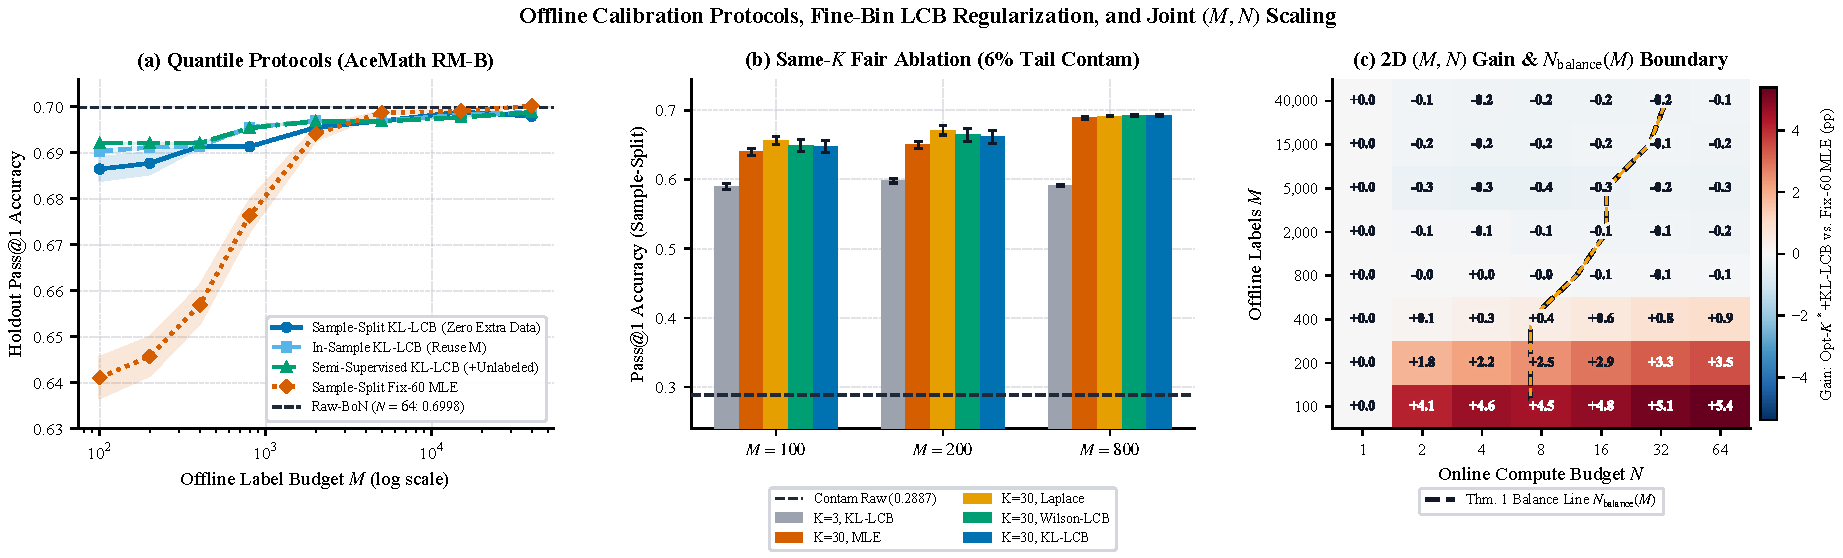
\includegraphics[width=0.84\textwidth]{fig2_joint_mn_and_protocols}
\caption{\textbf{Calibration protocols and $(M, N)$ regimes (\Cref{thm:joint-minimax,prop:spacings}).} \textbf{(a)} Holdout Pass@1 ($N=64$) across $M$ for Sample-Split, In-Sample, and Semi-Supervised $\mathrm{KL\text{-}LCB}$ vs.\ $\mathrm{Fix\text{-}60\ MLE}$ on \texttt{AceMath RM-B}. \textbf{(b)} Same-$K$ regularizer comparison under $6\%$ synthetic tail spikes ($\mathrm{Contam\ Raw}=0.2887$). \textbf{(c)} 2D $(M, N)$ gain of adaptive $K^*+\mathrm{KL\text{-}LCB}$ over $\mathrm{Fix\text{-}60\ MLE}$ (pp), overlaid with the theoretical balance threshold~\eqref{eq:n-balance}.}
\label{fig:joint-mn}
\end{figure}

\texttt{Sample-Split KL-LCB} (using $\beta=2$, $c_0 = 1.5$, $\delta_{\mathrm{cov}}=0.05$, and $K$ evaluated at $M/2$ in \Cref{prop:spacings}) sacrifices only $0.39\,\mathrm{pp}$ vs.\ In-Sample quantiles ($0.6864$ vs.\ $0.6903$) and $0.57\,\mathrm{pp}$ vs.\ Semi-Supervised quantiles ($0.6921$) at $M=100$---despite $M \in [100, 800]$ falling below \Cref{prop:spacings}'s conservative large-deviation threshold ($M_1+1 \ge 214\ln(16M)$)---outperforms \texttt{Fix-60 MLE} by $+4.53\,\mathrm{pp}$, and closes the gap for $M \ge 400$ (\texttt{GPQA-Qwen7B} in \texttt{Strategic-TTC} at $M=5{,}000$: $0.3063 / 0.3065 / 0.3081$). Crucially, on clean \texttt{AceMath RM-B}, all finite-bin calibrators in \Cref{tab:protocols} still trail uncalibrated \texttt{Raw-BoN} ($0.6998$) by at least $0.11\text{--}0.29\,\mathrm{pp}$ even at $M=5{,}000$ ($0.6969$--$0.6987$) due to within-bin tie coarsening. Across the full 2D $(M, N)$ grid (\Cref{fig:joint-mn}(c)), adaptive $K^*(M) + \mathrm{KL\text{-}LCB}$ beats $\mathrm{Fix\text{-}60\ MLE}$ by $+4.14$ to $+5.38\,\mathrm{pp}$ at $M=100$ ($N=2\dots 64$), $+1.82$ to $+3.46\,\mathrm{pp}$ at $M=200$, and $+0.14$ to $+0.95\,\mathrm{pp}$ at $M=400$, before saturating within $-0.35$ to $+0.03\,\mathrm{pp}$ once $M \ge 800$ crosses the balance line~\eqref{eq:n-balance}. Coarse-$K$ regularization drives clean-data gains, whereas isolating narrow $6\%$ tail spikes requires fine $K=30$ bins ($+6.4\text{--}7.4\,\mathrm{pp}$ over $K=3$), where LCB/Laplace beat same-$K$ MLE by $+1.2\text{--}2.8\,\mathrm{pp}$ while empirical Bernstein~\eqref{eq:eb-lcb} collapses ($0.6032$ vs.\ $0.6962$ at $M=400, K=20$).

\subsection{Disjoint Holdout Inference: Zero Clean-Data Gain and Risk Isolation}

Following \citet{nadeau2003inference}, \Cref{tab:single-split} evaluates a disjoint prompt split ($50/20/30$, primary split seed $830$) with frozen $\mathrm{Hybrid\text{-}Fixed}$ ($\varepsilon_{\mathrm{refit}} \equiv 0$, \Cref{alg:hybrid-fixed}) and two-sided paired studentized $t$-tests ($p_t$; exploratory 5-fold permutation checks use $+1$ smoothing \citep{phipson2010permutation}).

\begin{table}[htbp]
\centering
\caption{Disjoint $50/20/30$ primary results (bold marks row max; underline marks $\mathrm{Hybrid\text{-}Fixed}$). Notice $0.00\,\mathrm{pp}$ clean gain of $\mathrm{Hybrid\text{-}Fixed}$ over $\mathrm{Raw\text{-}BoN}$, confirming pure risk-control protection; the bottom row reports $\mathrm{Hybrid} - \mathrm{Raw}$ ($+0.55\,\mathrm{pp}$; $\mathrm{Hybrid} - \mathrm{Within\text{-}Z} = -0.32\,\mathrm{pp}$).}
\label{tab:single-split}
\footnotesize
\setlength{\tabcolsep}{2.8pt}
\begin{tabular}{lccccccc}
\toprule
Dataset & $P_{\mathrm{test}}$ ($N$) & Selected $\hat{m}$ & $\mathrm{Raw\text{-}BoN}$ & $\mathrm{Pooled}$ & $\mathrm{Within\text{-}Z}$ & $\mathrm{Hybrid}$ & $\Delta\text{ vs.\ Pool}\ (p_t)$ \\
\midrule
\texttt{S3 3-Domain}     & $839$ ($128$)   & $\mathrm{Raw\text{-}BoN}$ & $\mathbf{0.5159}$ & $0.4918$ & $0.5022$ & $\underline{\mathbf{0.5159}}$ & $+2.41\,\mathrm{pp}$ ($0.0050$) \\
\texttt{RB2 Skywork}     & $556$ ($4$)     & $\mathrm{Raw\text{-}BoN}$ & $\mathbf{0.8592}$ & $0.8409$ & $0.8500$ & $\underline{\mathbf{0.8592}}$ & $+1.83\,\mathrm{pp}$ ($0.0120$) \\
\texttt{AceMath RM-B}    & $2{,}695$ ($64$)& $\mathrm{Raw\text{-}BoN}$ & $0.7023$ & $\mathbf{0.7050}$ & $0.6733$ & $\underline{0.7023}$          & $-0.28\,\mathrm{pp}$ ($0.1400$) \\
\texttt{AceMath RM-A}    & $2{,}695$ ($64$)& $\mathrm{Raw\text{-}BoN}$ & $0.7358$ & $\mathbf{0.7365}$ & $0.7074$ & $\underline{0.7358}$          & $-0.07\,\mathrm{pp}$ ($0.6806$) \\
\texttt{OlympiadBench}   & $202$ ($128$)   & $\mathrm{Raw\text{-}BoN}$ & $0.4010$ & $\mathbf{0.4057}$ & $0.3141$ & $\underline{0.4010}$          & $-0.47\,\mathrm{pp}$ ($0.6742$) \\
\midrule
\texttt{college\_math RM-B} & $845$ ($64$) & $\mathrm{Pooled\text{-}LCB}$ & $0.4504$ & $0.4559$ & $\mathbf{0.4591}$ & \underline{$0.4559$} & $+0.55\,\mathrm{pp}$ vs.\ $\mathrm{Raw}$ ($0.1810$)$^*$ \\
\bottomrule
\end{tabular}
\vspace{2pt}
{\footnotesize $^*$Exploratory post-hoc candidate across 14 subset--RM pairs ($P=2{,}818$): peak $N=16$ ($0.4640$) $\to$ $N=64$ ($0.4579$, $-0.60 \pm 0.26\,\mathrm{pp}$, $p_{\mathrm{raw}} = 0.0208$, Bonferroni/Holm $p_{\mathrm{Bonf},14} = 0.2908$); 50/50 split check ($P_{\mathrm{conf}}=1{,}409$): $-1.08 \pm 0.38\,\mathrm{pp}, p_{\mathrm{conf}}=0.0048$.}
\end{table}

\paragraph{Honest Reading of \Cref{tab:single-split} and Statistical Power.}
On all five uncontaminated benchmark--verifier settings (\Cref{tab:single-split,fig:simpson}(a)), the minimal gate $\mathrm{Hybrid\text{-}Fixed}$ selects $\mathrm{Raw\text{-}BoN}$---achieving \textbf{$0.00\,\mathrm{pp}$ net improvement over $\mathrm{Raw\text{-}BoN}$}. Its empirical role on clean data is strictly risk containment: preventing Simpson confounding drops incurred by blind pooling on cross-domain mixtures (\texttt{S3}: $+2.41\,\mathrm{pp}, p_t=0.0050$; \texttt{RB2}: $+1.83\,\mathrm{pp}, p_t=0.0120$), and avoiding prompt-wise Z-score ceiling drops on math benchmarks ($-0.92$ to $-8.69\,\mathrm{pp}$ vs.\ $\mathrm{Raw\text{-}BoN}$; target-budget $\hat{\varepsilon}_{\mathrm{refit}} \in [0.0006, 0.0074]$, with overall max $0.0092$ on \texttt{OlympiadBench} at $N=16$). We also note finite-sample statistical power limits on smaller test sets (\texttt{OlympiadBench} $P_{\mathrm{test}}=202$ has paired SE $\approx 1.1\,\mathrm{pp}$ vs.\ $-0.47\,\mathrm{pp}$ difference). Across 14 uncontaminated \texttt{AceMath} subset--RM pairs, \texttt{college\_math RM-B} fails 14-family Bonferroni/Holm multiplicity correction ($p_{\mathrm{Bonf},14} = 0.2908$) and held-out testing ($0.4559$ vs.\ $\mathrm{Raw}\ 0.4504, p_t = 0.1810$; vs.\ $\mathrm{Within\text{-}Z}\ 0.4591$, $-0.32\,\mathrm{pp}$), serving strictly as an exploratory candidate (\Cref{fig:simpson}(b)). Note that \Cref{tab:pi0-ablation,tab:shift} below standardize on diagnostic split seed $835$ ($P_{\mathrm{test}}=2{,}695$), accounting for the slight baseline shift ($0.7083$ vs.\ $0.7023$).

\begin{figure}[tbp]
\centering
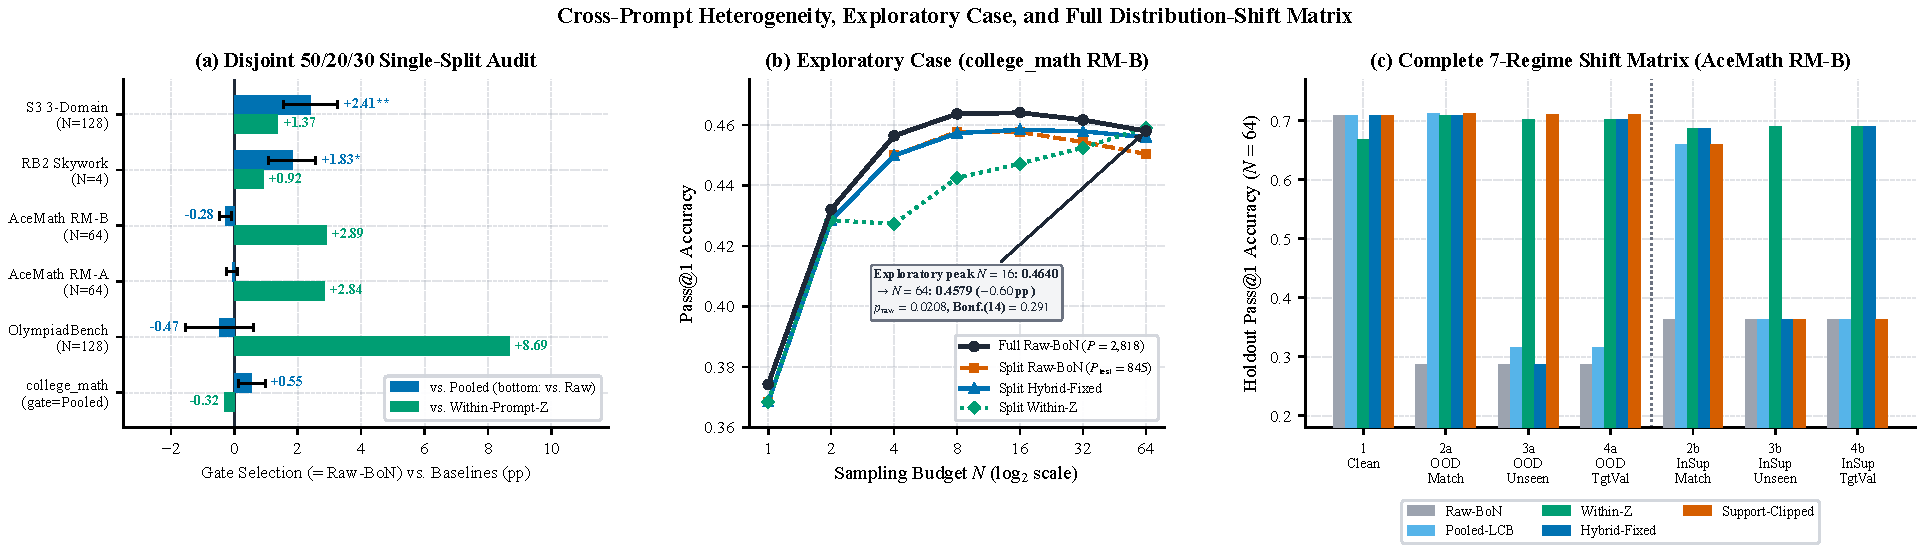
\includegraphics[width=0.91\textwidth]{fig3_heterogeneity_and_shift}
\caption{\textbf{Heterogeneity and shift (\Cref{sec:heterogeneity}).} \textbf{(a)} Disjoint 50/20/30 test gains of $\mathrm{Hybrid\text{-}Fixed}$ vs.\ $\mathrm{Pooled\text{-}LCB}$ and $\mathrm{Within\text{-}Prompt\text{-}Z}$ ($^{**}p_t<0.01, ^{*}p_t<0.05$). \textbf{(b)} Exploratory \texttt{college\_math RM-B} scaling curves (Bonf.\ $p=0.291$). \textbf{(c)} Complete 7-regime shift audit ($6\%$ out-of-distribution (OOD) vs.\ in-support $[q_{0.90}, q_{0.985}]$ contamination at $N=64$).}
\label{fig:simpson}
\end{figure}

\subsection{Empirical Boundary Audit for Theorem~\texorpdfstring{\ref{thm:sample-z-ceiling}}{3} and Counterfactual \texorpdfstring{$\hat{\pi}_0 = 0$}{pi0 = 0} Ablation}

To audit whether \Cref{thm:sample-z-ceiling} reflects real benchmark behavior beyond the idealized $\pi_1 = 0$ setting and whether empirical distributions match its Gaussian diagnostic assumptions, \Cref{tab:z-boundary-audit,fig:tmlr-z-diag} measure empirical boundary fractions $\hat{\pi}_0$ (all-wrong prompts), $\hat{\pi}_1$ (all-right prompts), predicted tail limit $\hat{L}_{\mathrm{tail}} = \frac{\hat{\pi}_1}{\hat{\pi}_0 + \hat{\pi}_1}$, sample Z-score class standard deviation ratio $\hat{\kappa}_Z := \hat{\sigma}_{Z,0}/\hat{\sigma}_{Z,1}$, non-Gaussianity diagnostics (tie rate, positive-class skewness, excess kurtosis), and $K=20$ equal-frequency sample-Z bin posteriors across all five benchmark--RM settings.

\paragraph{Synthetic Verification of Cases 1--4 and Empirical Diagnostic Audit.}
First, exact numerical evaluation at $N=4{,}096$ validates all four regimes of \Cref{thm:sample-z-ceiling} (\Cref{fig:tmlr-z-diag}(a)): (i) Case~1 ($\pi_0=0.45, \pi_1=0.10$) hits $L_{\mathrm{tail}}=0.1818$ with global peak $z^*=2.1664$ ($q_{\mathrm{pool},Z^*}(z^*)=0.5291$) and accuracy ceiling $0.5278 < 0.5447$ ($\mathrm{Raw\text{-}BoN}$; affine invariance discrepancy $4.44\times 10^{-16}$); (ii) Case~2 ($\pi_0=0.05, \pi_1=0.50, \mu_1=0.4$) shifts the global peak via adaptive right-tail search to $z^*=18.8111$ ($q_{\mathrm{peak}}=0.9680$), exhibits a shallow negative-side dip ($0.5233$ at $z \approx -3.68$) before rising strictly monotonically across $z \in [-3.6, 18.8]$, and shrinks the asymptotic $N\to\infty$ ceiling loss to $0.001345$ with exact zero finite-sample loss at $N=4{,}096$ ($\mathrm{Sample\text{-}Z} = \mathrm{Raw} = 0.6877$); (iii) Case~3 ($\pi_0=0, \pi_1=0.50$) attains $L_{\mathrm{tail}}=1.0$ and zero ceiling loss ($0.9932 = 0.9932$); and (iv) Case~4 ($\pi_0=0, \pi_1=0.10, \Delta=15$) demonstrates the \emph{Left-Tail Overtake Trap}: unconstrained two-sided maximization incurs an analytical asymptotic ceiling of $0.5500$ (loss $0.4500$) and stalls at $0.9427$ ($N=4{,}096$), whereas enforcing $Z \ge 0$ eliminates left-tail overtake and achieves full $1.0000 = \mathrm{Raw\text{-}BoN}$. Second, \Cref{tab:z-boundary-audit,fig:tmlr-z-diag}(b) bridge this Gaussian diagnostic mechanism to real non-Gaussian LLM logs (where within-prompt score ties reach $0.975$--$1.000$ on discrete/repeated math trajectories, positive-class excess kurtosis reaches $+7.55$ on \texttt{RB2} and $+28.14$ with skewness $-3.753$ on \texttt{OlympiadBench}, and $\hat{\kappa}_Z := \hat{\sigma}_{Z,0}/\hat{\sigma}_{Z,1} > 1$ across all five settings, ranging from $1.0563$ on \texttt{S3} to $1.3723$ on \texttt{OlympiadBench} in alignment with Z-induced variance inflation): four of five settings violate $\pi_1=0$ (\texttt{S3}: $\hat{\pi}_1=0.3149, \hat{L}_{\mathrm{tail}}=0.4900 \approx \hat{q}_Z(20)=0.4568$, moderating the drop to $-1.37\,\mathrm{pp}$), whereas \texttt{OlympiadBench} ($\hat{\pi}_0=0.2864, \hat{\pi}_1=0.1187, \hat{L}_{\mathrm{tail}}=0.2930$) collapses early from bin~$8/20$ ($0.6233$) to $0.2578$ at bin~$20/20$ ($41.59\%$ unsolvable-prompt candidates in the top $5\%$ $Z$-bin), driving the $-8.69\,\mathrm{pp}$ loss.

\begin{figure}[tbp]
\centering
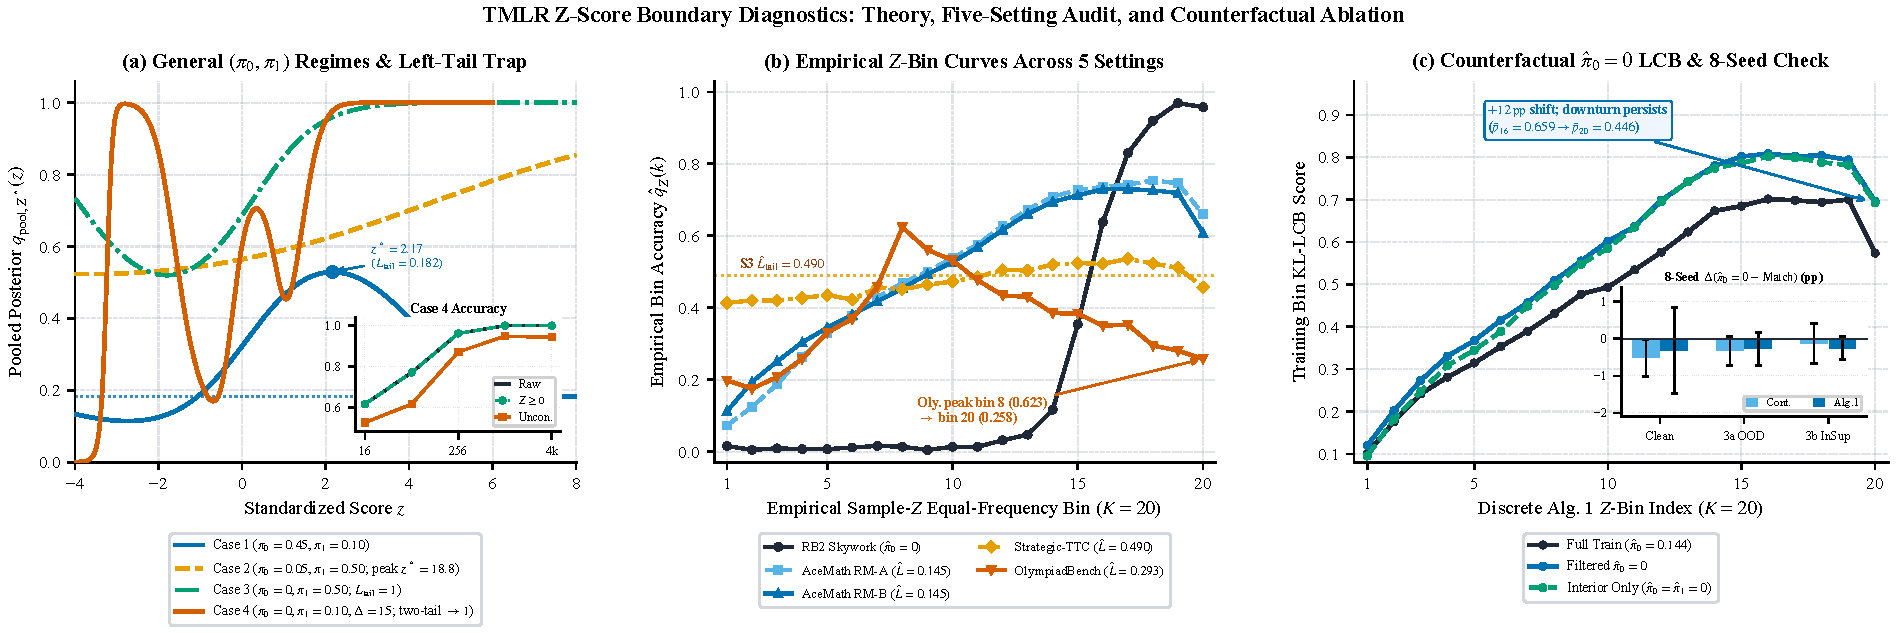
\includegraphics[width=0.86\textwidth]{fig5_tmlr_z_diagnostics}
\caption{\textbf{Z-score boundary diagnostics, empirical tail trajectories, and counterfactual $\hat{\pi}_0 = 0$ drift ablation (\Cref{thm:sample-z-ceiling}).} \textbf{(a)} Theoretical $q_{\mathrm{pool}, Z^*}(z)$ across general $(\pi_0, \pi_1)$ regimes: Case~1 ($\pi_0=0.45, \pi_1=0.10$, peak $z^*=2.17$, tail limit $L_{\mathrm{tail}}=0.182$), Case~2 ($\pi_0=0.05, \pi_1=0.50, \mu_1=0.4$; true peak pushed out to $z^*=18.81$), Case~3 ($\pi_0=0, \pi_1=0.50$; $L_{\mathrm{tail}}=1$), and Case~4 ($\pi_0=0, \pi_1=0.10, \Delta=15$; two-tail limit $1$), with the inset comparing Case~4 $N$-scaling accuracy ($N \in [16, 4096]$) under $\mathrm{Raw\text{-}BoN}$, unconstrained two-sided maximization (`Uncon.'), and right-half ($Z \ge 0$) maximization. \textbf{(b)} Empirical $K=20$ equal-frequency sample-$Z$ bin accuracies $\hat{q}_Z(k)$ across all five benchmark--verifier settings, overlaid with the \texttt{Strategic-TTC} tail limit $\hat{L}_{\mathrm{tail}}=0.490$ and the early peak collapse on \texttt{OlympiadBench} (bin~$8$: $0.623 \to$ bin~$20$: $0.258$). \textbf{(c)} Counterfactual \Cref{alg:split-kl-lcb} LCB bin curves across \texttt{AceMath RM-B} training splits (`Full`, `Filtered` $\hat{\pi}_0^{\mathrm{tr}}=0$, `Size-Matched`, and `Interior-Only`), highlighting the $\approx +12\,\mathrm{pp}$ baseline shift and persistent bin~$16 \to 20$ downturn, while the inset plots 8-seed mean $\pm$ SD test differences (`Filtered - Size-Matched`, pp) on Clean, 3a~OOD, and 3b~In-Support regimes.}
\label{fig:tmlr-z-diag}
\end{figure}

\begin{table}[tbp]
\centering
\caption{Empirical boundary-prompt proportions $(\hat{\pi}_0, \hat{\pi}_1)$, predicted tail ratio $\hat{L}_{\mathrm{tail}}$, $K=20$ sample-$Z$ bin posteriors, bin-20 zero-prompt share, tie rates, non-Gaussianity, class SD ratio $\hat{\kappa}_Z := \hat{\sigma}_{Z,0}/\hat{\sigma}_{Z,1}$, and 50/20/30 test $\mathrm{Within\text{-}Z} - \mathrm{Raw\text{-}BoN}$ drops (\Cref{thm:sample-z-ceiling}).}
\label{tab:z-boundary-audit}
\scriptsize
\setlength{\tabcolsep}{2.8pt}
\begin{tabular}{lcccccccccc}
\toprule
Benchmark ($P$, $N$) & $\hat{\pi}_0$ & $\hat{\pi}_1$ & $\hat{L}_{\mathrm{tail}}$ & $\max_k \hat{q}_Z$ (bin) & $\hat{q}_Z(20)$ & $\mathrm{Bin20}_0$ & $\mathrm{Tie}$ & $\mathrm{Skew}_+$ / $\mathrm{Kurt}_+$ & $\hat{\kappa}_Z$ & $\Delta_{Z-\mathrm{Raw}}$ \\
\midrule
\texttt{S3 3-Domain} ($2{,}798, 128$)    & $0.3277$ & $0.3149$ & $0.4900$ & $0.5357$ ($17/20$) & $0.4568$ & $0.3829$ & $1.000$ & $-0.30$ / $+0.68$  & $1.0563$ & $-1.37\,\mathrm{pp}$ \\
\texttt{RB2 Skywork} ($1{,}855, 4$)      & $0.0000$ & $0.0000$ & $\text{N/A}$ & $0.9687$ ($19/20$) & $0.9575$ & $0.0000$ & $0.009$ & $-0.40$ / $+7.55$  & $1.1767$ & $-0.92\,\mathrm{pp}$ \\
\texttt{AceMath RM-B} ($8{,}987, 64$)    & $0.1422$ & $0.0241$ & $0.1452$ & $0.7297$ ($17/20$) & $0.6079$ & $0.1619$ & $0.975$ & $-0.56$ / $+0.12$  & $1.2649$ & $-2.89\,\mathrm{pp}$ \\
\texttt{AceMath RM-A} ($8{,}987, 64$)    & $0.1422$ & $0.0241$ & $0.1452$ & $0.7534$ ($18/20$) & $0.6598$ & $0.1738$ & $0.978$ & $-0.63$ / $+0.36$  & $1.3525$ & $-2.84\,\mathrm{pp}$ \\
\texttt{OlympiadBench} ($674, 128$)      & $0.2864$ & $0.1187$ & $0.2930$ & $0.6233$ ($8/20$)  & $0.2578$ & $0.4159$ & $0.102$ & $-3.75$ / $+28.14$ & $1.3723$ & $-8.69\,\mathrm{pp}$ \\
\bottomrule
\end{tabular}
\end{table}

\paragraph{Counterfactual $\hat{\pi}_0 = 0$ Drift Ablation, Calibrator Semantics, and 8-Seed Check.}
To isolate the causal role of $\hat{\pi}_0 > 0$ prompts on \texttt{AceMath RM-B} ($P_{\mathrm{test}}=2{,}695, N=64$, seed $835$), \Cref{tab:pi0-ablation} removes all all-wrong training prompts ($\hat{\pi}_0^{\mathrm{train}} = 0$) and contrasts two distinct implementations while holding the prompt-level test splits fixed: (a) a \textbf{continuous piecewise-linear equal-frequency $\mathrm{KL\text{-}LCB}$ calibrator} (linearly interpolating bin KL-LCB anchors with no mid-bin tie-breaking loss), and (b) the \textbf{discrete \Cref{alg:split-kl-lcb} calibrator} using a candidate-level shuffled i.i.d.\ $50/50$ split ($M_1, M_2$) and uniform within-bin tie-breaking.

\begin{table}[htbp]
\centering
\caption{Counterfactual $\hat{\pi}_0 = 0$ training-set ablation on \texttt{AceMath RM-B} ($P_{\mathrm{test}}=2{,}695, N=64$, seed $835$; candidate-level shuffled i.i.d.\ $50/50$ split in \Cref{alg:split-kl-lcb}). Entries report continuous $\mathrm{Within\text{-}Z}$ accuracy [discrete \Cref{alg:split-kl-lcb} in brackets]. Clean $\mathrm{Raw}=0.7083$; 3a OOD $\mathrm{Raw}=0.2865$; 3b In-Support $\mathrm{Raw}=0.3627$.}
\label{tab:pi0-ablation}
\scriptsize
\setlength{\tabcolsep}{1.1pt}
\begin{tabular}{lccccccc}
\toprule
Train Regime ($P_{\mathrm{tr}}$) & $(\hat{\pi}_0^{\mathrm{tr}}, \hat{\pi}_1^{\mathrm{tr}})$ & Cont.\ Pk$\to$Tail & Alg.1 Pk$\to$Tail & $\bar{p}_{16}\!\to\!\bar{p}_{20}$ & Clean & 3a OOD & 3b InSup \\
\midrule
Full ($4{,}494$)            & $(0.1435, 0.0214)$ & $0.7074\!\to\!0.5881$ & $0.7016\!\to\!0.5739$ & $0.574\!\to\!0.370$ & $0.6690$ [$0.6726$] & $0.7024$ [$0.7013$] & $0.6907$ [$0.6901$] \\
Filtered $\hat{\pi}_0=0$ ($3{,}849$) & $(0.0000, 0.0249)$ & $0.8144\!\to\!0.7080$ & $0.8084\!\to\!0.6957$ & $0.659\!\to\!0.446$ & $0.6691$ [$0.6714$] & $0.7002$ [$0.7014$] & $0.6908$ [$0.6883$] \\
Size-Match ($3{,}849$)      & $(0.1468, 0.0216)$ & $0.7105\!\to\!0.5938$ & $0.7028\!\to\!0.5826$ & $0.578\!\to\!0.374$ & $0.6651$ [$0.6800$] & $0.6990$ [$0.7080$] & $0.6885$ [$0.6903$] \\
Interior ($3{,}753$)        & $(0.0000, 0.0000)$ & $0.8090\!\to\!0.7027$ & $0.8017\!\to\!0.6925$ & $0.649\!\to\!0.438$ & $0.6658$ [$0.6697$] & $0.6986$ [$0.7010$] & $0.6899$ [$0.6870$] \\
\bottomrule
\end{tabular}
\end{table}

\Cref{tab:pi0-ablation,fig:tmlr-z-diag}(c) establish a clear mechanistic explanation: removing $\hat{\pi}_0^{\mathrm{tr}}$ prompts shifts the right-tail LCB level upward by $\approx +12\,\mathrm{pp}$ for both calibrators ($0.5881 \to 0.7080$ continuous; $0.5739 \to 0.6957$ discrete \Cref{alg:split-kl-lcb}), yet a pronounced peak-to-tail downturn persists even when $\hat{\pi}_0^{\mathrm{tr}} = \hat{\pi}_1^{\mathrm{tr}} = 0$ ($0.8090 \to 0.7027$; \Cref{alg:split-kl-lcb} bin~$16 \to 20$ mean prompt prior $\bar{p}$ drops $0.659 \to 0.446$ under $\hat{\pi}_0=0$ and $0.649 \to 0.438$ under interior-only). Consequently, across 8 independent prompt split seeds (\texttt{101}--\texttt{835}), $\mathrm{Filtered}\ \hat{\pi}_0=0$ minus $\mathrm{Size\text{-}Matched}$ yields essentially unchanged generalization (mean $\pm$ SD: Clean $-0.51 \pm 0.50\,\mathrm{pp}$ [Alg.~1: $-0.31 \pm 1.15\,\mathrm{pp}$]; 3a~OOD $-0.33 \pm 0.40\,\mathrm{pp}$ [$-0.28 \pm 0.46\,\mathrm{pp}$]; 3b~In-Support $-0.13 \pm 0.54\,\mathrm{pp}$ [$-0.25 \pm 0.30\,\mathrm{pp}$]). This follows directly from $\tilde{\sigma}^2(p) = \sigma^2 + p(1-p)\Delta^2$: not only $p=0$, but also near-zero hard interior prompts ($p \in \{1/64, 2/64, \dots\}$) retain $v(p) \approx 1$ and continue concentrating in the extreme right $Z$-bins, sustaining tail-downturn robustness even without exact zero-prior prompts.

\subsection{Out-of-Support vs.\ In-Support Shift and Multi-RM Safety Tax}

Under $6\%$ wrong-trajectory spikes on \texttt{AceMath RM-B} ($P_{\mathrm{test}}=2{,}695, N=64$, seed $835$ aligned 1-to-1 with \Cref{tab:pi0-ablation}), \Cref{tab:shift,fig:simpson}(c) contrast \textbf{out-of-distribution (OOD) Spikes} ($> q_{0.995} + 0.8\sigma$) against \textbf{In-Support Contamination} ($[q_{0.90}, q_{0.985}]$, below the $99.8\%$ quantile cap), comparing the continuous piecewise-linear calibrator with discrete \Cref{alg:split-kl-lcb} (clipped at $-1$ per \Cref{alg:split-kl-lcb}).

\begin{table}[htbp]
\centering
\caption{Distribution-shift matrix on \texttt{AceMath RM-B} ($N=64, P_{\mathrm{test}}=2{,}695$, seed $835$) for OOD spikes vs.\ in-support $[q_{0.90}, q_{0.985}]$ contamination (brackets: discrete \Cref{alg:split-kl-lcb}; bold: continuous row best; underline: $\mathrm{Hybrid\text{-}Fixed}$).}
\label{tab:shift}
\scriptsize
\setlength{\tabcolsep}{1.6pt}
\begin{tabular}{llccccc}
\toprule
Regime (Train/Val $\to$ Test) & Val $\hat{m}$ & $\mathrm{Raw\text{-}BoN}$ & $\mathrm{Pooled\text{-}LCB}$ & $\mathrm{Within\text{-}Z}$ & $\mathrm{Hybrid\text{-}Fixed}$ & $\mathrm{Support\text{-}Clipped}$ \\
\midrule
1. Clean / Clean $\to$ Clean              & $\mathrm{Raw\text{-}BoN}$ [$\mathrm{Pooled}$]  & $0.7083$ & $\mathbf{0.7090}$ [$0.7096$] & $0.6690$ [$0.6726$] & \underline{$0.7083$} [$0.7096$] & $\mathbf{0.7090}$ [$0.7095$] \\
2a. OOD Contam Matched                    & $\mathrm{Within\text{-}Z}$                     & $0.2865$ & $\mathbf{0.7124}$ [$0.7099$] & $0.7093$ [$0.7076$] & \underline{$0.7093$} [$0.7076$] & $\mathbf{0.7124}$ [$0.7099$] \\
3a. OOD Unseen Shift                      & $\mathrm{Raw\text{-}BoN}$ [$\mathrm{Pooled}$]  & $0.2865$ & $0.3159$ [$0.3658$] & $0.7024$ [$0.7013$] & \underline{$0.2865$} [$0.3658$] & $\mathbf{0.7108}$ [$0.7105$] \\
4a. OOD Target Val Audit                  & $\mathrm{Within\text{-}Z}$                     & $0.2865$ & $0.3159$ [$0.3658$] & $0.7024$ [$0.7013$] & \underline{$0.7024$} [$0.7013$] & $\mathbf{0.7108}$ [$0.7105$] \\
\midrule
2b. In-Support Contam Matched             & $\mathrm{Within\text{-}Z}$                     & $0.3627$ & $0.6599$ [$0.6421$] & $\mathbf{0.6868}$ [$0.6909$] & \underline{$\mathbf{0.6868}$} [$0.6909$] & $0.6599$ [$0.6421$] \\
3b. In-Support Unseen Shift               & $\mathrm{Raw\text{-}BoN}$ [$\mathrm{Pooled}$]  & $0.3627$ & $0.3629$ [$0.3876$] & $\mathbf{0.6907}$ [$0.6901$] & \underline{$0.3627$} [$0.3876$] & $0.3629$ [$0.3875$] \\
4b. In-Support Target Val Audit           & $\mathrm{Within\text{-}Z}$                     & $0.3627$ & $0.3629$ [$0.3876$] & $\mathbf{0.6907}$ [$0.6901$] & \underline{$\mathbf{0.6907}$} [$0.6901$] & $0.3629$ [$0.3875$] \\
\bottomrule
\end{tabular}
\vspace{2pt}
{\scriptsize \emph{Note:} On clean validation (Regimes~1, 3a, 3b), continuous validation selects $\mathrm{Raw\text{-}BoN}$ ($0.7083$), whereas discrete \Cref{alg:split-kl-lcb} selects $\mathrm{Alg1\text{-}Pooled}$ ($0.7096 > 0.7083$), matching bracketed $\mathrm{Hybrid\text{-}Fixed}$ test accuracies [$0.7096$], [$0.3658$], and [$0.3876$].}
\end{table}

While $\mathrm{Support\text{-}Clipped}$ stops unseen OOD spikes (3a: $0.7108$; discrete \Cref{alg:split-kl-lcb}: $0.7105$), it collapses nearly identically to $\mathrm{Raw\text{-}BoN}$ under unseen \emph{in-support} contamination (3b: $0.3629$ / $0.3875$ vs.\ $0.3627$) because adversarial candidates remain below the $99.8\%$ quantile cap. In that regime, only target validation auditing (4b) switches to $\mathrm{Within\text{-}Prompt\text{-}Z}$ to recover $0.6907$ ($+32.80\,\mathrm{pp}, p_t < 10^{-215}$). In Regime~2a, both continuous ($\mathrm{Within\text{-}Z}$, $0.7093$) and discrete ($\mathrm{Alg1\text{-}Within\text{-}Z}$, $0.7076$) selectors win on matched OOD validation and remain within $0.31\,\mathrm{pp}$ of $\mathrm{Pooled\text{-}LCB}$ ($0.7124$ / $0.7099$).

\begin{figure}[htbp]
\centering
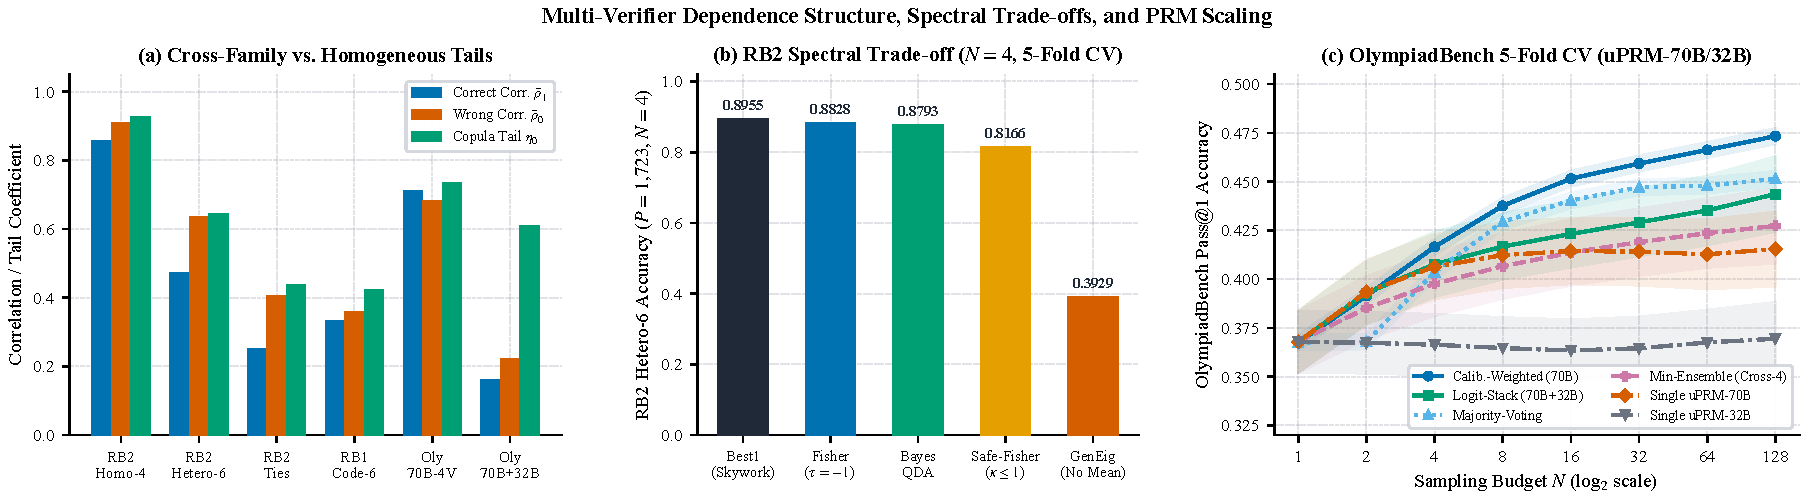
\includegraphics[width=0.84\textwidth]{fig4_multi_rm_dependence}
\caption{\textbf{Multi-verifier dependence, spectral trade-offs, and PRM scaling (\Cref{sec:ensemble}).} \textbf{(a)} Cross-family vs.\ homogeneous wrong/correct correlations $(\bar{\rho}_1, \bar{\rho}_0)$ and Gaussian-Copula residual tail index $\eta_0$ across \texttt{RB1}, \texttt{RB2}, and \texttt{OlympiadBench}. \textbf{(b)} \texttt{RB2 Hetero-6} 5-fold CV spectral paths ($P=1{,}723, N=4$), showing unconstrained $\mathrm{Fisher}$ and $\mathrm{Bayes\ QDA}$ vs.\ conservative $\mathrm{Safe\text{-}Fisher}(\kappa \le 1)$ and SNR-blind $\mathrm{GenEig}$. \textbf{(c)} \texttt{OlympiadBench} 5-fold CV PRM scaling ($P=674$), comparing $\mathrm{Cal\text{-}Vote}$ and $\mathrm{Logit\text{-}Stack}$ against single-PRM baselines (\texttt{70B}/\texttt{32B}) and conservative $\mathrm{Min\text{-}Ensemble}$.}
\label{fig:multi-rm}
\end{figure}

\paragraph{Multi-Verifier Correlation Structure and Conservative ``Safety Tax''.}
\Cref{fig:multi-rm} corroborates \Cref{sec:ensemble}: homogeneous \texttt{RB2} models share strong wrong-answer correlation ($\bar{\rho}_0 = 0.9088, \eta_0 = 0.9284$ on \texttt{RB2 Homo-4}), whereas cross-family RMs decouple errors ($\bar{\rho}_0 = 0.6359, \eta_0 = 0.6437$ on \texttt{RB2 Hetero-6}; $\bar{\rho}_0 = 0.2221$ across \texttt{uPRM-70B+32B}). For the $3\times 3$ zero-KKT matrix
\[
\Sigma = \begin{pmatrix}1 & 0 & 0.5\\ 0 & 1 & 0.5\\ 0.5 & 0.5 & 1\end{pmatrix} \qquad \Big(|I_{+,c}|=2,\ I_{0,c}=\{3\},\ \gamma_c=2,\ \theta_{c, I_0}=\tfrac{1}{2}\Big),
\]
the exact tail survival function $\bar{F}_{\min}(t) = \Prob(M_{\min} > t)$ matches $\frac{1}{4\pi}t^{-2}e^{-t^2}$ at $t=500$ with ratio $1.0022$. Crucially, however, 5-fold cross-validation in \Cref{fig:multi-rm}(b)--(c) (subject to fold-overlap variance underestimation per \citet{nadeau2003inference}) reveals the exact multi-RM analogue of our single-verifier findings:
On \texttt{RB2 Hetero-6} ($P=1{,}723$ prompts with four candidates each, $N=4$), unconstrained $\mathrm{Fisher}(\tau=-1)=0.8828$ and $\mathrm{Bayes\ QDA}=0.8793$ beat $\mathrm{Safe\text{-}Fisher}(\kappa\le 1)=0.8166$ ($-6.62\,\mathrm{pp}$, while still beating SNR-blind $\mathrm{GenEig}=0.3929$). Similarly, on non-collapsing \texttt{OlympiadBench} ($P=674, N=128$), calibrated weighted voting reaches $0.4733$ and $\mathrm{Logit\text{-}Stack}$ reaches $0.4436$ (vs.\ \texttt{70B} $0.4154$, \texttt{32B} $0.3694$), whereas tail-hardened $\mathrm{Min\text{-}Ensemble}$ is overly conservative. Just as finite-bin LCB incurs a small tax relative to uncalibrated $\mathrm{Raw\text{-}BoN}$ on clean monotone pools, enforcing asymptotic $\kappa \le 1$ tail-safety or worst-case $\min$ constraints levies a predictable ``safety tax'' when real budgets ($N=4$) or verifier tails are already well behaved.

\section{Discussion and Limitations}
\label{sec:discussion}

\paragraph{Practical Takeaways.}
(1) \emph{Do not blindly replace monotone verifiers on clean benchmarks:} uncalibrated $\mathrm{Raw\text{-}BoN}$ avoids binning tie-loss and cross-prompt Simpson confounding, and $\mathrm{Hybrid\text{-}Fixed}$ achieves $0.00\,\mathrm{pp}$ clean gain precisely because it preserves $\mathrm{Raw\text{-}BoN}$ unless contamination appears.
(2) \emph{Jointly scale calibration labels $M$ with compute $N$:} pushing compute beyond $N_{\mathrm{balance}}(M) \asymp (M/\ln M)^{\frac{1}{2\beta+1}}$ hits the offline statistical ceiling.
(3) \emph{Do not rely on prompt-wise Z-scores alone or clean-only validation:} Z-standardization loses $-0.92$ to $-8.69\,\mathrm{pp}$ across all five clean benchmark--verifier settings via low-prior and boundary tail competition (\Cref{thm:sample-z-ceiling,tab:z-boundary-audit}), while unseen \emph{in-support} contamination defeats outlier clipping (\Cref{tab:shift}), making small target-domain validation audits essential.
(4) \emph{Understand asymptotic constraints as insurance, not free gains:} $\mathrm{Safe\text{-}Fisher}$ and $\mathrm{Min\text{-}Ensemble}$ pay an accuracy tax in low-$N$ or non-collapsing pools.

\paragraph{Limitations.}
Five methodological and empirical boundaries qualify our results: (1) our minimax bounds assume 1D conditional continuous marginals on a fixed prompt distribution, whereas real benchmarks exhibit massive discrete score ties (up to $100\%$ on \texttt{Strategic-TTC} and $>97.5\%$ on \texttt{AceMath}) and heavy positive-class non-Gaussianity (kurtosis $+28.14$ and skewness $-3.75$ on \texttt{OlympiadBench}); (2) our tail-collapse ablations inject synthetic $6\%$ OOD and in-support wrong-answer spikes because current clean benchmarks rarely trigger severe uncalibrated degradation at tested budgets; (3) quantile support clipping protects only against out-of-range spikes and fails under unseen in-support contamination (\Cref{tab:shift}), while holdout gating partitions prompts statically rather than performing instance-level per-prompt routing; (4) our multi-verifier Gaussian and Copula tail laws are parametric asymptotic criteria rather than distribution-free finite-sample bounds, and the 5-fold cross-validation curves in \Cref{fig:multi-rm}(b)--(c) remain subject to fold-overlap variance underestimation \citep{nadeau2003inference}; and (5) smaller evaluation subsets such as \texttt{OlympiadBench} ($P_{\mathrm{test}}=202$) limit statistical power to detect sub-percentage differences in single-split comparisons.

\paragraph{Reproducibility.}
All experiments execute deterministically on CPU with fixed seeds on cached public evaluation logs (\Cref{app:index}, \Cref{tab:index}).
\ifdefined\USEPREPRINT
Code, verification tests, and figure/paper build scripts are available at \url{https://github.com/6Riemann9/test-time-scaling-theory} (Zenodo code archive DOI: \texttt{10.5281/zenodo.24563479}; earlier preprint DOI: \texttt{10.5281/zenodo.24563692}; author ORCID: \href{https://orcid.org/0009-0007-5524-7050}{0009-0007-5524-7050}).
\else
An anonymized code and verification archive is provided with the supplementary material to reproduce every theorem, table, and figure.
\fi

\subsubsection*{Broader Impact Statement}
Understanding when verifier calibration improves or harms test-time scaling has direct practical value for building reliable inference pipelines: it prevents practitioners from wasting validation data or incurring silent accuracy drops when applying pooled calibration across mixed domains or sample-Z normalization on unsolvable-heavy benchmarks. Moreover, cross-prompt pooling and prompt-wise $\mathrm{Within\text{-}Z}$ normalization can induce a hidden subgroup fairness squeeze: harder or underrepresented reasoning cohorts with higher unsolvable mass ($\hat{\pi}_0$) or lower baseline pass rates systematically concentrate in distorted score regions and absorb disproportionate accuracy losses when deployed without subgroup-level auditing. At the same time, our distribution-shift audit carries clear safety implications: naive outlier clipping offers a false sense of security against adversarial or distributionally shifted false positives whose scores lie inside normal operating quantiles (\Cref{tab:shift}, Regime~3b). Safety-critical deployments should therefore combine conservative selection gates with ongoing target-domain validation monitoring and multi-source verification rather than trusting unverified OOD clipping or static offline fits.

\ifdefined\USEPREPRINT
\subsubsection*{Acknowledgments}
This work uses publicly released reward-model and reasoning benchmark evaluation logs without external API queries or proprietary funding conflicts.
\fi

\bibliography{references_tmlr}
\bibliographystyle{tmlr}

\newpage
\appendix
\counterwithin{theorem}{section}
\counterwithin{proposition}{section}

\section{Single-Verifier Preliminaries}
\label{app:preliminaries}

For completeness, we summarize and prove the single-verifier preliminary statements used in \Cref{sec:model}.

\begin{theorem}[Exact Order-Statistic Integral with Tie Atoms]
\label{thm:app-pit}
Let $F_1, F_0$ be arbitrary CDFs on $\R$ with countable atom set $\mathcal{A}$, mixture $\Fmix = p F_1 + (1-p)F_0$, and uniform random tie-breaking on $\mathcal{I}_{\max}$. Then~\eqref{eq:pit-exact} holds for all $N \ge 1$, with $q(a) = \frac{p\Delta F_1(a)}{\Delta\Fmix(a)}$ at $a \in \mathcal{A}$. For Gaussian $S \mid Y=c \sim \mathcal{N}(\mu_c, \sigma_c^2)$, $P_{\mathrm{BoN}}(2) - p = p(1-p)[2\Phi(\frac{\mu_1-\mu_0}{\sqrt{\sigma_1^2+\sigma_0^2}}) - 1]$ and $P_{\mathrm{Anti\text{-}BoN}}(2) = 2p - P_{\mathrm{BoN}}(2)$.
\end{theorem}
\begin{proof}
At any atom $a \in \mathcal{A}$, conditional correctness of a uniformly chosen tied maximizer equals $q(a)$, while $\Prob(S_{(N)} = a) = [\Fmix(a)]^N - [\Fmix(a-)]^N = \Delta([\Fmix]^N)(a)$. Pushforward equivalence with $v \mapsto \Fmix^{-1}(v^{1/N})$ follows from the Galois connection $\Fmix^{-1}(u) \le x \iff u \le \Fmix(x)$.
\end{proof}

\begin{theorem}[Heavy Wrong-Tail Collapse, $C^1/C^0$ Monotone Likelihood Ratio Property ($\mathrm{MLRP}$), and Fixed-Peak Gumbel Constant]
\label{thm:app-collapse}
Let $F_1, F_0$ have positive densities $f_1, f_0$ on an open interval $I$ with right endpoint $x_R$, and for any measurable subset $A \subseteq I$ with $\Prob(S \in A) > 0$, denote restricted conditional accuracy by $P_{\mathrm{BoN}}(N; A) := \Prob(Y_{\hat{i}^*} = 1 \mid S_{1:N} \in A^N)$.
\begin{enumerate}[leftmargin=1.8em,itemsep=2pt]
    \item If $\lim_{x\uparrow x_R} f_1(x)/f_0(x) = 0$, then $\lim_{N\to\infty} P_{\mathrm{BoN}}(N) = 0$ and $\arg\max_{N\ge 1} P_{\mathrm{BoN}}(N)$ is finite.
    \item Under $f_1, f_0 \in C^1(I)$ (over closed subintervals $[a,b] \subset I$) or $f_1, f_0 \in C^0(I)$ (over unions of two disjoint closed intervals $I_1 \cup I_2 \subset I$), $P_{\mathrm{BoN}}(N+1; A) \ge P_{\mathrm{BoN}}(N; A)$ holds for all $p \in (0, 1), N \ge 1$ iff $\Lambda(x) = f_1(x)/f_0(x)$ is non-decreasing on $I$. For Gaussians with $\kappa = \sigma_0/\sigma_1 < 1$ and $\Delta\mu = 0$, $P_{\mathrm{BoN}}(1) = P_{\mathrm{BoN}}(2) = p$ followed by strict increase $P_{\mathrm{BoN}}(N) \uparrow 1$ for $N \ge 2$.
    \item \textbf{(Fixed-Peak-Height Gumbel Limit)} For Gaussian $\sigma_0 = \kappa\sigma_1$ ($\kappa > 1$) under $\Delta\mu(\kappa) := \sigma_1\sqrt{c_1(\kappa^2-1)}$ ($c_1 > 0$), let $x_{\mathrm{peak}} = \frac{\mu_1\sigma_0^2 - \mu_0\sigma_1^2}{\sigma_0^2 - \sigma_1^2}$, $\tau^{-2} = \sigma_1^{-2} - \sigma_0^{-2}$, $N_0^* = 1/\barFmix(x_{\mathrm{peak}})$, $N^*_{\mathrm{exact}} \in \arg\max_{N\ge 1} P_{\mathrm{BoN}}(N)$, and $h = \fmix(x_{\mathrm{peak}})/\barFmix(x_{\mathrm{peak}})$, where $\sigma(u) = (1+e^{-u})^{-1}$ and $\gamma \approx 0.577216$ is the Euler--Mascheroni constant. As $\kappa \downarrow 1^+$, $q_{\mathrm{peak}}(\kappa) \to \sigma(\logit(p) + c_1/2) \in (0, 1)$, $h(\kappa)\tau(\kappa) \sim \frac{\sqrt{c_1}}{\kappa^2 - 1} \to +\infty$, and $\frac{2(h\tau)^2}{q_{\mathrm{peak}}(1-q_{\mathrm{peak}})}(q_{\mathrm{peak}} - \E[q(S_{(e^\delta N_0^*)})]) \to (\delta + \gamma)^2 + \frac{\pi^2}{6}$ uniformly on $[-D, D]$, yielding $\lim_{\kappa \downarrow 1^+} N^*_{\mathrm{exact}} / N_0^* = e^{-\gamma} \approx 0.561459$.
\end{enumerate}
\end{theorem}
\begin{proof}
Parts (1)--(2) follow from Stieltjes integration by parts $P_{\mathrm{BoN}}(N+1)-P_{\mathrm{BoN}}(N) = \int \Fmix^N(1-\Fmix)\,dq$ and the two-interval identity $P_{\mathrm{BoN}}(2; I_1\cup I_2) - P_{\mathrm{BoN}}(1; I_1\cup I_2) \to -w_1^* w_2^*(q(x_1)-q(x_2)) < 0$ when $q(x_1) > q(x_2)$ ($x_1 < x_2$). For (3), setting $\mu_0 = 0$ gives $x_{\mathrm{peak}} = \frac{\kappa^2\sigma_1\sqrt{c_1}}{\sqrt{\kappa^2-1}}$, $h \sim \frac{\sqrt{c_1}}{\sigma_1\sqrt{\kappa^2-1}}$, $\tau = \frac{\kappa\sigma_1}{\sqrt{\kappa^2-1}}$, and log-odds constant $L_0(\kappa) := \logit(p) + \ln\kappa + c_1/2 \to \logit(p) + c_1/2$. Writing $q(x_{\mathrm{peak}}+y) = g(y^2/(2\tau^2))$ with $g(u) = \sigma(L_0(\kappa) - u)$ bounds the fourth-order Taylor remainder on $|y| \le \sqrt{2}\tau$. The normalized maximum $G_N = h(S_{(N_\delta)} - x_{\mathrm{peak}}) - \delta$ converges in distribution and fourth moments to $\mathrm{Gumbel}(0,1)$ via monotone normal hazard bounds and left-tail truncation at $a := \frac{1}{2}x_{\mathrm{peak}}$; Karlin single-crossing unimodality locks $N^*_{\mathrm{exact}}/N_0^* \to e^{-\gamma}$.
\end{proof}

\begin{theorem}[Binary Verifier Scaling and Calibrated Weighted Majority]
\label{thm:app-cal}
(i) For binary $S_i \in \{0,1\}$ whose true positive rate $\alpha = \mathrm{TPR}$ exceeds its false positive rate $\beta_{\mathrm{fp}} = \mathrm{FPR}$, with selection rate $q_1 = p\alpha + (1-p)\beta_{\mathrm{fp}}$ and positive predictive value $\mathrm{PPV} = p\alpha/q_1$, $P_{\mathrm{BoN,bin}}(N) = \mathrm{PPV} - C(1-q_1)^N$ where $C = \frac{p(1-p)(\alpha-\beta_{\mathrm{fp}})}{q_1(1-q_1)}$; letting $P_N = \mathrm{Bernoulli}(P_{\mathrm{BoN,bin}}(N))$ and $\delta_1$ denote a point mass at $1$, when $\beta_{\mathrm{fp}} = 0$ ($\mathrm{PPV}=1$) we have $\DKL(P_N \| \delta_1) = +\infty$ while $\TV(P_N, \delta_1) = \frac{1-p}{1-p\alpha}(1-p\alpha)^N$ and $\DKL(\delta_1 \| P_N) = \Theta((1-p\alpha)^N)$. (ii) Consider discrete answer output $A_i$ taking the correct answer $a^*$ w.p.\ $p$ and countably many wrong answers $\{a_j\}_{j\ge 1}$ w.p.\ $p_j$ ($\sum_j p_j = 1-p$), weighted by bounded scores $W_i = w(S_i) \in [0, w_{\max}]$ with conditional means $\mu_{w,+} := \E[W_i \mid A_i=a^*]$ and $\mu_{w,j} := \E[W_i \mid A_i=a_j]$, selecting $\hat{A}_N := \arg\max_a \sum_{i: A_i = a} W_i$. If $\Delta_{\min} := p\mu_{w,+} - \sup_j(p_j\mu_{w,j}) > 0$, there exist $K_0 \ge 1$ and $c > 0$ such that grouping the tail $\sum_{j>K_0}p_j < \frac{p\mu_{w,+}}{2w_{\max}}$ into a super-bucket yields $\Prob(\hat{A}_N \neq a^*) \le (K_0+1)e^{-c N}$.
\end{theorem}
\begin{proof}
Part (i) decomposes over the all-negative event $\{S_{1:N} = \mathbf{0}\}$ of probability $(1-q_1)^N$, noting $\delta_1$ assigns zero mass to $0$. In (ii), because $\sum_{j>K_0} p_j \mu_{w,j} \le w_{\max}\sum_{j>K_0} p_j < \frac{1}{2}p\mu_{w,+}$, applying Hoeffding's inequality to each bounded sum $W_i(\ind\{A_i=a^*\} - \ind\{A_i=a_j\})$ for $1 \le j \le K_0$ and once to the tail super-bucket $\bigcup_{j>K_0}\{a_j\}$ gives the $(K_0+1)$-term exponential union bound.
\end{proof}

\section{Proofs for Section~\texorpdfstring{\ref{sec:minimax}}{4} (Joint Minimax and Spacings)}
\label{app:minimax}

\begin{proof}[Proof of \Cref{thm:joint-minimax}]
\textbf{Part 1:} On $\mathcal{F}_\beta^{\mathrm{sep}}$, for $\varepsilon \in (0, \varepsilon_\eta)$, $\{x : q(x) > q^* - \varepsilon\} \subset U_\eta$ gives $\bar{F}_Q(q^* - \varepsilon) = (1+o(1))\frac{2f^*}{C^{1/\beta}}\varepsilon^{1/\beta}$; substituting $u = N^\beta\varepsilon$ and dominated convergence yield $\frac{\Gamma(\beta+1)C}{(2f^*)^\beta}N^{-\beta}$.

\textbf{Part 2:} For $K > \frac{2}{\eta_0 f_{\min}}$, any equal-frequency bin inside $U_{\eta_0}$ has width $\le \frac{1}{K f_{\min}} < \frac{\eta_0}{2}$. Let $i^{\mathrm{near}} = \arg\min_{1\le i\le N}|S_i - x^*|$, $D_N = |S_{i^{\mathrm{near}}} - x^*|$, $k^{\mathrm{near}} = k(S_{i^{\mathrm{near}}})$, and $\hat{k}^* = k(S_{\hat{i}^*})$. Conditioning on $\mathcal{F}_{\mathrm{bins}} = \sigma(\mathcal{D}_M, k(S_1),\dots,k(S_N))$ with strictly uniform tie-breaking gives $\E[Y_{\hat{i}^*} \mid \mathcal{F}_{\mathrm{bins}}] = q_{\hat{k}^*}$. Define three offline bad events, each of probability $\le \frac{1}{3M}$: $\mathcal{B}_1 = \{\exists k: \hat{s}_k^{\mathrm{KL\text{-}LCB}}(\frac{1}{3M}) > q_k\}$ (Cram\'er--Chernoff + union bound), $\mathcal{B}_2 = \{\exists k: m_k < \frac{M}{2K}\}$ (multiplicative Chernoff for $M \ge 8K\ln(3KM)$), and $\mathcal{B}_3 = \{\exists k: m_k \ge 1,\ q_k - \hat{q}_k > \sqrt{\frac{\ln(3KM)}{2m_k}}\}$ (conditional Hoeffding). Let $\mathcal{B}_{\mathrm{miss}} = \{D_N > \eta_0/2\}$, which has probability $\le (1 - \eta_0 f_{\min})^N \le e^{-\eta_0 f_{\min}N}$. On $\mathcal{G} = (\mathcal{B}_1 \cup \mathcal{B}_2 \cup \mathcal{B}_3 \cup \mathcal{B}_{\mathrm{miss}})^c$, $B_{k^{\mathrm{near}}} \subset U_{\eta_0}$ and $(a+b)^\beta \le c_\beta(a^\beta + b^\beta)$ yield $q^* - q_{k^{\mathrm{near}}} \le C_1 c_\beta D_N^\beta + \frac{C_1 c_\beta}{(K f_{\min})^\beta}$. By $\mathcal{B}_1^c, \mathcal{B}_2^c, \mathcal{B}_3^c$ and Pinsker's inequality $\KL(\hat{q}_k, \hat{s}_k^{\mathrm{KL\text{-}LCB}}) \ge 2(\hat{q}_k - \hat{s}_k^{\mathrm{KL\text{-}LCB}})^2$,
\[
q_{\hat{k}^*} \ge \hat{s}_{\hat{k}^*}^{\mathrm{KL\text{-}LCB}} \ge \hat{s}_{k^{\mathrm{near}}}^{\mathrm{KL\text{-}LCB}} \ge q_{k^{\mathrm{near}}} - 2\sqrt{\frac{\ln(3KM)}{2m_{k^{\mathrm{near}}}}} \ge q_{k^{\mathrm{near}}} - 2\sqrt{\frac{K\ln(3KM)}{M}}.
\]
Integrating $\E[\ind_{\mathcal{G}}D_N^\beta] \le \int_0^{\eta_0/2}\beta r^{\beta-1}e^{-2f_{\min}Nr}\,dr \le \frac{\Gamma(\beta+1)}{(2f_{\min})^\beta}N^{-\beta}$ yields~\eqref{eq:joint-upper}.

\textbf{Part 3:} Place uniform density $\fmix \equiv f_0 \ge f_{\min}$ on an interval $I_0$ of length $L_0 \in (2\eta_0, 1/f_{\min})$ (assigning remaining mass $1 - f_0 L_0 > 0$ smoothly outside $I_0$, valid since $2\eta_0 f_{\min} < 1$), and construct $J = \Theta(h^{-1})$ disjoint bumps $q_j(x) = \frac{1}{2} + a_\beta h^\beta\max(0, 1 - |x-t_j|^\beta/h^\beta)$ strictly inside $I_0$ with bump scale $a_\beta \in (0, C_1]$. Because unlabeled $S_{1:N}$ drawn from the common marginal $\fmix$ carry zero information about $j$, $\DKL(P_j^{\otimes M}\otimes\Fmix^{\otimes N} \| P_0^{\otimes M}\otimes\Fmix^{\otimes N}) = M\DKL(P_j\|P_0) \le C_2 M h^{2\beta+1}$. Choosing $h \asymp (\frac{\ln M}{M})^{\frac{1}{2\beta+1}}$ and Fano's inequality gives $\Omega((\frac{\ln M}{M})^{\frac{\beta}{2\beta+1}})$; evaluating at $P^* \in \mathcal{F}_\beta^{\mathrm{unif}} \cap \mathcal{F}_\beta^{\mathrm{sep}}$ gives $\Omega(N^{-\beta})$ by Part~1.
\end{proof}

\begin{proof}[Proof of \Cref{prop:spacings}]
By continuity of $\Fmix$ and Pyke's representation \citep{pyke1965spacings}, $(\hat{\pi}_1,\dots,\hat{\pi}_K) \stackrel{d}{=} (G_1/G_{\mathrm{tot}},\dots,G_K/G_{\mathrm{tot}})$ where $G_k \sim \mathrm{Gamma}(d_k, 1)$ and $G_{\mathrm{tot}} \sim \mathrm{Gamma}(M_1+1, 1)$ with $\frac{11}{12}\frac{M_1+1}{K} \le d_k \le \frac{13}{12}\frac{M_1+1}{K}$ when $M_1+1 \ge 12K$. For $\psi(c) = c - 1 - \ln c$, $\min(\psi(0.60), \psi(1.65)) \approx 0.11082 > \frac{1}{9.1}$ and $\min(\psi(0.90), \psi(1.10)) \approx 0.0046898 > \frac{1}{214}$. Thus $d_{\min} \ge 9.1\ln(16KM)$ and $M_1+1 \ge 214\ln(16M)$ ensure $G_k \in [0.60 d_k, 1.65 d_k]$ ($\forall k$) and $G_{\mathrm{tot}} \in [0.90(M_1+1), 1.10(M_1+1)]$ w.p.\ $\ge 1 - \frac{1}{4M}$, giving $\frac{0.60\times 11/12}{1.10 K} = \frac{1}{2K} \le \hat{\pi}_k \le \frac{1.65\times 13/12}{0.90 K} = \frac{143}{72K} < \frac{2}{K}$. Conditioning on $\mathcal{D}_{M_1}^{\mathrm{edge}}$, $M_2 \ge 16K\ln(4KM)$ yields $\Prob(\exists k: m_k < \frac{M_2}{4K} \mid \mathcal{D}_{M_1}^{\mathrm{edge}}) \le \frac{1}{4M}$. Substituting $m_k \ge \frac{M_2}{4K} \ge \frac{M}{8K}$ into $\sqrt{\frac{2\ln(4KM)}{m_k}} \le 4\sqrt{\frac{K\ln(4KM)}{M}}$ completes the proof.
\end{proof}

\section{Proofs for Section~\texorpdfstring{\ref{sec:heterogeneity}}{5} (Prompt Heterogeneity and General-\texorpdfstring{$(\pi_0,\pi_1)$}{(pi0, pi1)} Sample-\texorpdfstring{$Z_{i,N}$}{Z\_i,N})}
\label{app:heterogeneity}

\begin{proof}[Proof of \Cref{thm:simpson}]
Differentiating $w(x\mid s) = f_{\mathrm{mix},x}(s)/f_{\mathrm{pool}}(s)$ gives $\partial_s w(x\mid s) = w(x\mid s)(g_x(s) - \E[g_X(s)\mid S=s])$, establishing (1). For (2), on $s \in [3.5, 4.2]$:
\begin{enumerate}[leftmargin=1.8em,itemsep=2pt]
    \item $\ell'_1(s) = -0.75(s - 0.4) \in [-2.85, -2.325] < 0$ and $\ell'_2(s) = -0.75(s - 3.4) \in [-0.60, -0.075] < 0$. Hence $q_1, q_2$ decrease strictly on $[3.5, 4.2]$, locking $q_1(s) \in [4.750\times 10^{-4},\, 2.900\times 10^{-3}]$ and $q_2(s) \in [0.96810,\, 0.97464]$, so $q_2(s) - q_1(s) > 0.96519$. Since $u \mapsto u(1-u)$ decreases strictly on $(0.5, 1)$, $\partial_s q_2(s) \le -0.075\, q_2(3.5)(1-q_2(3.5)) \approx -1.8539\times 10^{-3} < -1.85\times 10^{-3}$ and $|\partial_s q_2(s)| \le 0.60\, q_2(4.2)(1-q_2(4.2)) < 0.01915$, while $\partial_s q_1(s) < -1.10\times 10^{-3}$ and $|\partial_s q_1(s)| < 0.00827$, giving $|\E[\partial_s q_X(s)\mid S=s]| < 0.01915$.
    \item All four Gaussian means $\{0.3, 0.0, 3.3, 3.0\} < 3.5$, so $r(s) = \frac{0.15 f_{\mathrm{mix},2}(s)}{0.85 f_{\mathrm{mix},1}(s)} \in [1.1211, 3.2180]$ and $w_1(s)w_2(s) = \frac{r(s)}{(1+r(s))^2} \ge \frac{3.2180}{4.2180^2} > 0.18087$.
    \item Component convex combinations give $g_1(s) \le -0.25 s$ and $g_2(s) \ge -(s - 3.3)$, so $g_2(s) - g_1(s) \ge 3.3 - 0.75 s \ge 3.3 - 0.75\times 4.2 = +0.15$.
\end{enumerate}
Multiplying yields $\Cov(Y, g_X(s)\mid S=s) > 0.18087\times 0.96519\times 0.15 > 0.02618$, so $q'_{\mathrm{pool}}(s) > 0.02618 - 0.01915 = +7.03\times 10^{-3}$ (more precisely $+7.044\times 10^{-3}$) $> 0$ for all $s \in [3.5, 4.2]$.
\end{proof}

\begin{proof}[Proof of \Cref{prop:zscore-n2,thm:sample-z-ceiling,prop:hybrid}]
In \Cref{prop:zscore-n2}(1), for any fixed $i \ge 1$, the SLLN gives $\bar{\tilde{S}}_N \xrightarrow{\mathrm{a.s.}} \tilde{\mu}(X)$ and $\hat{\tilde{s}}_N \xrightarrow{\mathrm{a.s.}} \tilde{\sigma}(X) > 0$, whence $Z_{i,N} \xrightarrow{\mathrm{a.s.}} Z_i^*(X)$. In (2), exchangeability gives $P_{\mathrm{Cal\text{-}BoN}}^{\mathrm{oracle}}(2) - P_{\mathrm{Raw}}(2) = 2\E[(q_X(S_1)-q_X(S_2))\ind\{S_1<S_2, q_X(S_1)>q_X(S_2)\}]$ and symmetrically for $\mathrm{Anti\text{-}BoN}(2)$, proving the bidirectional characterization.

For \Cref{thm:sample-z-ceiling}(1), on any boundary stratum $p \in \{0,1\}$ we have $\tilde{\sigma}(p) = \sigma$, so $Z^* \mid \{p(X)=c\} \sim \mathcal{N}(0, 1)$ with standard normal density $\phi(z)$. On interior strata $p \in [p_{\min}, p_{\max}]$, $\tilde{\sigma}^2(p) = \sigma^2 + p(1-p)\Delta^2$, giving conditional Gaussian variance $v(p) := \sigma^2 / \tilde{\sigma}^2(p) \le v_{\max} < 1$; therefore every interior component density decays as $o(\phi(z))$ as $z \to \pm\infty$. Dividing positive mixture density by total mixture density yields $\lim_{z\to\pm\infty} q_{\mathrm{pool}, Z^*}(z) = \frac{\pi_1}{\pi_0 + \pi_1} = L_{\mathrm{tail}}$.
In Case~(1a) ($\pi_0 = 0, \pi_1 > 0$), $L_{\mathrm{tail}} = 1 > q_{\mathrm{pool}, Z^*}(z)$ for all $z \in \R$ (interior strata supply positive negative-label density everywhere). Because $\lim_{z\to -\infty} q_{\mathrm{pool}, Z^*}(z) = 1$ as well, when heterogeneous interior priors have large $\Delta/\sigma$ (e.g., Case~4 in \Cref{fig:tmlr-z-diag}(a)), $q_{\mathrm{pool}, Z^*}$ can approach $1$ more steeply along $z \to -\infty$ than along moderate $z > 0$, allowing unconstrained two-sided maximization $\max_{1\le i\le N} q_{\mathrm{pool}, Z^*}(Z_{i,N})$ to select a negative order statistic $Z_{i,N} \ll 0$ where interior prompt accuracy vanishes. Restricting optimization to the non-empty right half $\{i : Z_{i,N} \ge 0\}$ rules out the left tail: since $\Delta_N(x) := \max_{1\le i\le N}|Z_{i,N} - Z_i^*(x)| \xrightarrow{p} 0$, $\max_i Z_{i,N} \ge \max_i Z_i^*(x) - \Delta_N(x) \xrightarrow{p} +\infty$ while $Z_{i,N} \ge 0 \implies Z_i^*(x) \ge -\Delta_N(x)$ prevents selecting from the far left tail ($z \ll 0$); because $q_{\mathrm{pool}, Z^*}(z) < 1$ on compacts $[-\eta, M_Z]$ and tends to $1$ as $z \to +\infty$, selection on $\{i : Z_{i,N} \ge 0\}$ forces $Z_{\hat{i}_N^{\ge 0}}^*(x) \xrightarrow{p} +\infty$ for $\mathcal{P}_X$-a.e.\ $x$, so bounded convergence gives $\lim_{N\to\infty} P_{\mathrm{Sample\text{-}Z\text{-}Cal}}^{\mathrm{right\text{-}half}}(N) = 1 = P_{\mathrm{Raw}}(\infty)$.
In Case~(1b) ($\pi_0 > 0, \pi_1 \ge 0$, $\Prob(p(X)\in(0,1)) > 0$), notice $L_{\mathrm{tail}} < 1$. Because interior prompts are compactly supported on $[p_{\min}, p_{\max}] \subset (0, 1)$, $\logit\big(\tilde{q}_X(\tilde{\mu}(X) + \tilde{\sigma}(X)z)\big) \ge \logit(p_{\min}) - \frac{\Delta^2}{2\sigma^2} + \frac{\Delta}{\sigma} z \to +\infty$ holds uniformly over all $p \in [p_{\min}, p_{\max}]$, so choosing $z_0$ sufficiently large guarantees $\tilde{q}_X(\tilde{\mu}(X) + \tilde{\sigma}(X)z_0) > L_{\mathrm{tail}}$ uniformly across all interior prompts; hence $q_{\mathrm{pool}, Z^*}(z_0)$ is a strictly convex combination of $L_{\mathrm{tail}}$ and the strictly larger interior average, yielding $q_{\mathrm{pool}, Z^*}(z_0) > L_{\mathrm{tail}}$. By continuity and $\lim_{z\to\pm\infty} q_{\mathrm{pool}, Z^*}(z) = L_{\mathrm{tail}}$, the global maximizer set $K^* := \arg\max_{z\in\R} q_{\mathrm{pool}, Z^*}(z)$ is non-empty and compact, $K^* \subset [-M_Z, M_Z]$.

For \Cref{thm:sample-z-ceiling}(2), by location--scale invariance $Z_{i,N} = (\tilde{S}_i - \bar{\tilde{S}}_N)/\hat{\tilde{s}}_N$ cancels $(b(X), a(X))$. Fixing $X=x$, sub-Gaussianity yields $\max_{1\le i\le N}|Z_i^*(x)| = O_p(\sqrt{\ln N})$, $|\bar{\tilde{S}}_N - \tilde{\mu}(x)| = O_p(N^{-1/2})$, and $|\hat{\tilde{s}}_N - \tilde{\sigma}(x)| = O_p(N^{-1/2})$, so $\Delta_N(x) = O_p(\sqrt{(\ln N)/N}) \xrightarrow{p} 0$. Since $q_{\mathrm{pool}, Z^*}$ is uniformly continuous and stays below $q_Z^*$ outside compacts around $K^*$, $\operatorname{dist}(Z_{\hat{i}_N}^*(x), K^*) \xrightarrow{p} 0$. By exact affine invariance, $\Prob(Y_{\hat{i}_N}=1 \mid X=x) = \E[\tilde{q}_x(\tilde{\mu}(x) + \tilde{\sigma}(x)Z_{\hat{i}_N}^*(x)) \mid X=x]$, which equals $0$ when $p(x)=0$, $1$ when $p(x)=1$, and stays strictly below $1$ on $K^*$ for every interior prompt $p(x) \in (0, 1)$. Passing $\limsup_{N \to \infty}$ inside $\E_X[\cdot]$ via \textbf{Reverse Fatou's Lemma} (valid for bounded random variables even when $|K^*|\ge 2$ prevents pointwise limits) yields $\limsup_{N\to\infty} P_{\mathrm{Sample\text{-}Z\text{-}Cal}}^{\mathrm{oracle}}(N) \le \pi_1 + \E_X[\max_{z\in K^*} \tilde{q}_X(\tilde{\mu}(X)+\tilde{\sigma}(X)z)\,\ind\{p(X)\in(0,1)\}] < \pi_1 + (1 - \pi_0 - \pi_1) = 1 - \pi_0 = P_{\mathrm{Raw}}(\infty)$.

For \Cref{prop:hybrid}, conditional on $\mathcal{D}_{\mathrm{train}}$, each $m \in \mathcal{M}$ evaluates i.i.d.\ $[0,1]$-valued per-prompt indicators on $\mathcal{D}_{\mathrm{val}}$ ($\frac{1}{4M_{\mathrm{val}}}$-sub-Gaussian deviation $\Delta_m := \hat{A}_{\mathrm{val}}(m) - A_{\mathrm{fixed}}(m)$), so Hoeffding's inequality over $2|\mathcal{M}|$ events gives the $1-\delta$ bound $2\sqrt{\frac{\ln(2|\mathcal{M}|/\delta)}{2 M_{\mathrm{val}}}}$, while $A_{\mathrm{fixed}}(m^*) - A_{\mathrm{fixed}}(\hat{m}) \le -\Delta_{m^*} + \max_{m\in\mathcal{M}}\Delta_m$ together with $\E_{\mathrm{val}}[\Delta_{m^*}]=0$ and Massart's finite-class maximal inequality gives expected regret $\le \sqrt{\frac{2\cdot (1/(4 M_{\mathrm{val}}))\ln|\mathcal{M}|}{1}} = \sqrt{\frac{\ln|\mathcal{M}|}{2 M_{\mathrm{val}}}}$. Part (2) adds $|A_{\mathrm{refit}}(m^*) - A_{\mathrm{fixed}}(m^*)| + |A_{\mathrm{fixed}}(\hat{m}) - A_{\mathrm{refit}}(\hat{m})| \le 2\varepsilon_{\mathrm{refit}}$ by the triangle inequality.
\end{proof}

\section{Proofs for Section~\texorpdfstring{\ref{sec:ensemble}}{6} (Multi-Verifier Ensembles)}
\label{app:ensemble}

\begin{proof}[Proof of \Cref{thm:gaussian-ensemble,thm:copula}]
\textbf{Theorem~\ref{thm:gaussian-ensemble}(1):} Since $\mathbf{w}^\top \mathbf{S} \mid Y=c \sim \mathcal{N}(\mathbf{w}^\top \boldsymbol{\mu}_c, \mathbf{w}^\top \Sigma_c \mathbf{w})$, asymptotic convergence to $1$ requires $\frac{\mathbf{w}^\top \Sigma_0 \mathbf{w}}{\mathbf{w}^\top \Sigma_1 \mathbf{w}} < 1$ (or $=1$ with $\mathbf{w}^\top \Delta\boldsymbol{\mu} > 0$), which by the Rayleigh quotient under $P^\top \Sigma_1 P = I_K$ and $P^\top \Sigma_0 P = \operatorname{diag}(\lambda_1,\dots,\lambda_K)$ holds iff $\lambda_{\min} < 1$ (or $\lambda_{\min}=1$ with positive mean separation in $V_{\min}$). For the $N=2$ constrained objective, setting $\mathbf{v} = P^{-1}\mathbf{w}$ and $x_k = v_k^2 \ge 0$ normalizes the denominator $\mathbf{w}^\top(\Sigma_1+\Sigma_0)\mathbf{w} = \sum_{k=1}^K (1+\lambda_k) x_k = 1$ by scale invariance, converting maximization of $\SNR_2(\mathbf{w})$ into maximizing the strictly concave function $\sum_{k=1}^K |d_k|\sqrt{x_k}$ subject to the linear inequality $\sum_{k=1}^K (\lambda_k - \kappa_{\max}^2)x_k \le 0$ and $\sum_{k=1}^K (1+\lambda_k)x_k = 1$. Under Slater condition $\lambda_{\min} < \kappa_{\max}^2 < R(\mathbf{w}_{\mathrm{Fisher}})$, strong duality holds. At any interior stationary point with $\alpha > 0, \mu \ge 0$, KKT stationarity gives $\frac{|d_k|}{2\sqrt{x_k}} = \alpha(1+\lambda_k) + \mu(\lambda_k - \kappa_{\max}^2)$, recovering $\mathbf{w}_\tau = (\Sigma_0 - \tau\Sigma_1)^{-1}\Delta\boldsymbol{\mu}$ with $\tau = -\frac{\alpha - \mu\kappa_{\max}^2}{\alpha + \mu} \in [-1, \lambda_{\min})$. Differentiating $R(\mathbf{w}_\tau) = C(\tau)/D(\tau)$ gives $R'(\tau) < 0$ by Cauchy--Schwarz ($C(\tau)^2 < A(\tau)D(\tau)$). When $P_{V_{\min}}\mathbf{d} \neq \mathbf{0}$, $\lim_{\tau\uparrow\lambda_{\min}^-} R(\mathbf{w}_\tau) = \lambda_{\min} < \kappa_{\max}^2$, guaranteeing a unique interior $\tau^* \in (-1, \lambda_{\min})$. Conversely, when $P_{V_{\min}}\mathbf{d} = \mathbf{0}$ and $\lim_{\tau\uparrow\lambda_{\min}^-} R(\mathbf{w}_\tau) \ge \kappa_{\max}^2$, the objective ignores $k \in I_{\min}$, so dual multiplier $\tau^* = \lambda_{\min}$ allows adding zero-objective mass $\alpha\mathbf{u}_{\min} \in P V_{\min}$ (normalized by $\mathbf{u}_{\min}^\top \Sigma_1 \mathbf{u}_{\min} = 1$, i.e., $\|P^{-1}\mathbf{u}_{\min}\|_2 = 1$, with $v_k^\perp := (P^{-1}\mathbf{w}_{\lambda_{\min}^-})_k$) via $\mathbf{w}^* = \mathbf{w}_{\lambda_{\min}^-} + \alpha\mathbf{u}_{\min}$ solving $\sum_{k \notin I_{\min}}(\lambda_k - \kappa_{\max}^2)(v_k^\perp)^2 =\allowbreak \alpha^2(\kappa_{\max}^2 - \lambda_{\min})$ so that $R(\mathbf{w}^*) = \kappa_{\max}^2$. For Bayes QDA under $\Sigma_0 \succ \Sigma_1$, $q_{\mathrm{Bayes}}(\mathbf{s})$ attains a unique global maximum $q^*_{\mathrm{Bayes}} < 1$ with negative-definite Hessian, so level sets $\{q_{\mathrm{Bayes}} > q^*_{\mathrm{Bayes}} - u\}$ are $K$-dimensional ellipsoids of volume $(1+o(1))c_K u^{K/2}$ (with local ellipsoid volume prefactor $c_K > 0$), yielding excess regret $\Theta(N^{-2/K})$.

\textbf{Theorem~\ref{thm:gaussian-ensemble}(2):} Differentiating $\Prob(M_{\min}(\mathbf{S}) > t \mid Y=c)$ gives $f_{\min, c}(t) = \sum_{k=1}^K \phi_{c,k}(t)\Prob(\mathbf{S}_{-k} > t\mathbf{1}_{K-1} \mid S^{(k)}=t, Y=c)$, representing probability flux across the $K$ orthant faces (where $\phi_{c,k}$ is the univariate marginal normal density of $S^{(k)} \mid Y=c$). For inactive faces $k \in J_c$, complementary slackness enforces $u_{c,k}^* > 1$, so the restricted minimum quadratic form exceeds $\gamma_c$ by a strict margin $\Delta\gamma > 0$, making their contribution exponentially smaller $O(e^{-\Delta\gamma t^2/2})$. On essential faces $k \in I_{+,c}$, changing variables in the orthogonal subspace via $s_j - t = \xi_j / (t w_{c,j})$ (for $j \in I_{+,c} \setminus \{k\}$) isolates the quadratic exponent $-\frac{\gamma_c}{2}t^2 + \beta_c t$ and $|I_{+,c}|-1$ exponentially decaying half-line factors $\prod_{j \in I_{+,c}\setminus\{k\}} w_{c,j}^{-1}$, while the KKT identity $\Sigma_{c, I_{0,c}I_{+,c}}\Sigma_{c, I_{+,c}I_{+,c}}^{-1}\mathbf{1}_{I_{+,c}} = \mathbf{1}_{I_{0,c}}$ cancels all $O(t)$ drift on weakly active coordinates $I_{0,c}$, which converge in distribution to the Schur-complement Gaussian $\mathbf{W}_{I_{0,c}} \sim \mathcal{N}(\tilde{\boldsymbol{\mu}}_{0|+},\tilde{\Sigma}_{0|+})$ and contribute the positive constant $\theta_{c,I_0} = \Prob(\mathbf{W}_{I_{0,c}} > \mathbf{0}) \in (0, 1]$ instead of extra $t^{-1}$ powers. Summing over $k \in I_{+,c}$ with $\gamma_c = \sum_{k\in I_{+,c}} w_{c,k}$ yields $f_{\min,c}(t) = (1+o(1))\gamma_c C_c^{\mathrm{sf}} t^{1-|I_{+,c}|}e^{-\frac{\gamma_c}{2}t^2+\beta_c t}$, whereas weakly active faces $k \in I_{0,c}$ retain all $|I_{+,c}|$ compressed coordinates and contribute $O(t^{-|I_{+,c}|}e^{-\frac{\gamma_c}{2}t^2+\beta_c t}) = o(f_{\min,c}(t))$.

\textbf{Theorem~\ref{thm:copula}:} Writing $Z_k = h_c(t) := \Phi^{-1}(F_{t_{\alpha_c}}((t-\mu_c)/\sigma_c))$ transforms $\Prob(M_{\min} > t \mid Y=c, \text{non-shock}) = \Prob(\min_k Z_k > h_c(t))$. Since $h_c(t) = \sqrt{2\alpha_c \ln t}(1+o(1))$ satisfies $e^{-h_c(t)^2/2} = \Theta(t^{-\alpha_c}(\ln t)^{1/2})$ and $h_c'(t) = \Theta(t^{-1}(\ln t)^{-1/2})$, substituting $h_c(t)$ into the Gaussian minimum density of Theorem~\ref{thm:gaussian-ensemble}(2) ($\boldsymbol{\mu}=\mathbf{0}, \Sigma_c = R_c$) multiplies $e^{-\gamma_c h_c(t)^2/2} h_c(t)^{1-|I_{+,c}|} h_c'(t) = \Theta\big(t^{-\alpha_c/\eta_c - 1}(\ln t)^{(\gamma_c(R_c)-|I_{+,c}|)/2}\big)$ with $\eta_c = 1/\gamma_c(R_c)$. For $K \ge 2$ and $R_c \succ 0$, optimizing over any $2\times 2$ principal submatrix gives $\gamma_c(R_c) \ge 2/(1 + \rho_{12}) > 1$, so $\eta_c \in (0, 1)$. Under $(R_c)_{ij} \ge 0$, Slepian's lemma implies $\min_{\mathbf{u}\ge \mathbf{1}} \mathbf{u}^\top R_c^{-1}\mathbf{u} \le K$ (giving $\eta_c \ge 1/K$), while the block-diagonal matrix $\operatorname{diag}(R_{-0.2}, R_{+0.5})$ gives $\gamma_c = \frac{2}{0.8} + \frac{2}{1.5} = \frac{23}{6}$ and hence $\eta_c = \frac{6}{23} > \frac{1}{4}$ despite negative entries, proving elementwise non-negativity is unnecessary. Finally, when $\epsilon_s > 0$, the comonotonic branch contributes $\epsilon_s \Theta(t^{-\alpha_0 - 1})$ ($\eta_{0,\mathrm{eff}} = 1$), dominating wrong tails whenever $\alpha_0 < \alpha_1$ and forcing collapse to $0$; when $\epsilon_s = 0$, comparing survival/density ratios yields the stated main-exponent and log-factor trichotomy.
\end{proof}

\section{Benchmark Specifications and Experimental Protocols}
\label{app:index}

\Cref{tab:index} summarizes all public evaluation benchmarks, sample sizes, candidate budgets, split designs, and seed counts used across our empirical audit. All experiments run deterministically on a single CPU from cached public verifier score logs without external API calls.

\begin{table}[htbp]
\centering
\caption{Benchmark specifications and empirical evaluation protocols across all experiments.}
\label{tab:index}
\scriptsize
\setlength{\tabcolsep}{3pt}
\begin{tabular}{@{}lcclll@{}}
\toprule
Benchmark / Pool & $P$ & $N$ & Verifier(s) & Protocol / Seeds & Scope \\
\midrule
\texttt{AceMath-RB} & $8{,}987$ & $64$ & Official \texttt{RM-A}, \texttt{RM-B} & \parbox[t]{3.4cm}{\raggedright 50-rep $(M,N)$; 50/20/30 (8 seeds); 7-shift} & \parbox[t]{3.9cm}{\raggedright Sec.~7.1--7.4; Tables~\ref{tab:protocols}--\ref{tab:shift}; Figs.~\ref{fig:joint-mn}, \ref{fig:simpson}, \ref{fig:tmlr-z-diag}} \\
\addlinespace[2pt]
\texttt{Strategic-TTC} (\texttt{S3}) & $2{,}798$ & $128$ & \parbox[t]{3.2cm}{\raggedright Outcome RM (\texttt{GSM8K+GPQA+AIME})} & \parbox[t]{3.4cm}{\raggedright 50/20/30 split; $K=20$ $Z$-bin} & \parbox[t]{3.9cm}{\raggedright Sec.~7.1--7.3; Tables~\ref{tab:single-split}, \ref{tab:z-boundary-audit}; Figs.~\ref{fig:simpson}(a), \ref{fig:tmlr-z-diag}(b)} \\
\addlinespace[2pt]
\texttt{OlympiadBench} & $674$ & $128$ & \texttt{uPRM-70B}, \texttt{uPRM-32B} & \parbox[t]{3.4cm}{\raggedright 50/20/30 split; 5-fold CV (Fig.~\ref{fig:multi-rm}(c))} & \parbox[t]{3.9cm}{\raggedright Sec.~7.2--7.4; Tables~\ref{tab:single-split}, \ref{tab:z-boundary-audit}; Figs.~\ref{fig:simpson}(a), \ref{fig:tmlr-z-diag}(b), \ref{fig:multi-rm}(c)} \\
\addlinespace[2pt]
\texttt{reward-bench-2} & $1{,}855$ ($1{,}723$) & $4$ & \parbox[t]{3.2cm}{\raggedright \texttt{Skywork} + 6 hetero / 4 homo} & \parbox[t]{3.4cm}{\raggedright 50/20/30 split; 5-fold CV (Fig.~\ref{fig:multi-rm}(b))} & \parbox[t]{3.9cm}{\raggedright Sec.~7.2--7.4; Tables~\ref{tab:single-split}, \ref{tab:z-boundary-audit}; Figs.~\ref{fig:simpson}(a), \ref{fig:tmlr-z-diag}(b), \ref{fig:multi-rm}(a)--(b)} \\
\addlinespace[2pt]
\texttt{reward-bench-1} & $2{,}985$ & $2$ & \parbox[t]{3.2cm}{\raggedright 6 Code RMs (incl.\ \texttt{DeBERTa})} & $(\bar{\rho}_1, \bar{\rho}_0, \eta_0)$ dependence audit & Sec.~7.4; Fig.~\ref{fig:multi-rm}(a) \\
\bottomrule
\end{tabular}
\end{table}

\ifdefined\USEPREPRINT
\paragraph{Artifact Traceability Map.}
{\raggedright\footnotesize
For preprint readers inspecting the accompanying open-source repository:
\begin{itemize}[leftmargin=1.4em,itemsep=1pt,topsep=2pt]
\item \Cref{thm:joint-minimax,prop:spacings} map to \texttt{src/\allowbreak tts\_theory/\allowbreak calibration\_theory.py} (\texttt{tight\_\allowbreak joint\_\allowbreak minimax\_\allowbreak scaling}, \texttt{empirical\_\allowbreak quantile\_\allowbreak spacings\_\allowbreak bounds}).
\item \Cref{thm:simpson,prop:zscore-n2,thm:sample-z-ceiling,prop:hybrid} map to \texttt{src/\allowbreak tts\_theory/\allowbreak heterogeneity\_theory.py} (\texttt{diagnose\_\allowbreak simpson\_\allowbreak confounding}, \texttt{diagnose\_\allowbreak zscore\_\allowbreak induced\_\allowbreak collapse}, \texttt{verify\_\allowbreak sample\_\allowbreak zscore\_\allowbreak extremal\_\allowbreak convergence}) and \texttt{src/\allowbreak tts\_theory/\allowbreak real\_eval.py}.
\item \Cref{thm:gaussian-ensemble,thm:copula} map to \texttt{src/\allowbreak tts\_theory/\allowbreak ensemble\_theory.py} (\texttt{solve\_\allowbreak positive\_\allowbreak quadrant\_\allowbreak qp}), while \Cref{thm:app-pit,thm:app-collapse,thm:app-cal} map to \texttt{src/\allowbreak tts\_theory/\allowbreak theorems.py}, \texttt{integrals.py}, and \texttt{algorithms.py}.
\item Scripts \texttt{scripts/\allowbreak verify\_\allowbreak v9\_\allowbreak consolidation.py} and \texttt{scripts/\allowbreak verify\_\allowbreak v10\_\allowbreak release.py} regenerate \Cref{tab:protocols,tab:single-split} and \Cref{fig:overview,fig:joint-mn,fig:simpson,fig:multi-rm}; \texttt{scripts/\allowbreak verify\_\allowbreak tmlr\_\allowbreak diagnostics.py} exclusively regenerates \Cref{tab:z-boundary-audit,tab:pi0-ablation,tab:shift} and \Cref{fig:tmlr-z-diag} (under the candidate-level shuffled i.i.d.\ 50/50 split and $-1$ clip protocol); and \texttt{scripts/\allowbreak plot\_\allowbreak tmlr\_\allowbreak figures.py} exports all TMLR vector figures.
\end{itemize}\par}
\fi

\end{document}
